\documentclass{article}

\usepackage{wrapfig}
\usepackage{amsfonts}
\usepackage[all]{xy}
\usepackage{amssymb}
\usepackage{amsmath}
\usepackage{mathrsfs}
\usepackage{amsthm}
\usepackage{enumerate}
\usepackage[hidelinks]{hyperref}
\usepackage{ulem}
\usepackage{tikz}  
\usetikzlibrary{arrows.meta}%画箭头用的包
\usetikzlibrary{cd}
\usepackage{multicol} %用于实现在同一页中实现不同的分栏

\usepackage{geometry}
% \geometry{a4paper,left=2cm,right=2cm,top=2cm,bottom=2cm}
% \geometry{a4paper,left=1cm,right=1cm,top=1cm,bottom=1cm}

\newtheorem{defn}{Definition}[subsection]
\newtheorem{prop}[defn]{Proposition}
\newtheorem{lem}[defn]{Lemma}
\newtheorem{thm}[defn]{Theorem}
\newtheorem{cor}[defn]{Corollary}
\newtheorem{rmk}[defn]{Remark}
\newtheorem{claim}[defn]{Claim}
\newtheorem{const}[defn]{Construction}
\newtheorem{fact}[defn]{Fact}
\newtheorem{problem}{Problem}
\newtheorem*{ques}{Question}

% \setcounter{section}{0}

\title{Sarkisov program}
\author{wyz}
\date{\today}

\begin{document}

  \maketitle
  \tableofcontents
  %\newpage
\section{Introduction}

The purpose of this article is to show that two different log Mori fibre spaces as outputs of a klt pair can be linked by composition of  Sarkisov links.

\subsection{Motivation and Main theorem}
% Start with a projective log smooth pair $ \left(X,B\right) $, and assume we can run $ (K_X+B)$-MMP on it. The program may have different results, and the relation of the outputs is defined below:
The \textbf{Minimal model program (MMP)}  aims to classify varieties up to birational equivalent classed, by finding a minimal model all or Mori fibre space. Let $ \left(X,B\right) $ be a (klt or lc) pair, and assume we can run $ (K_X+B)$-MMP on it. Note that the varieties appear in the program are called \textbf{results} of the MMP, and the varieties where the MMP ends are called the \textbf{output} of the MMP.
\begin{enumerate}
  \item If $\kappa(X,B)\geqslant 0$, then we expected that MMP ends with a \textbf{minimal model}, i.e. a birational map $X \dashrightarrow Y$ such that $(K_Y+B_Y)$ is nef;
  \item If $\kappa(X,B)= -\infty$, then we expected that MMP ends with a log Mori fibre space, i.e. a birational map $X \dashrightarrow Y$ and a contraction $Y\to S$ such that $\dim Y<\dim X$ and $-(K_Y+B_Y)$ is relative ample.
\end{enumerate}
However, for each case the output may not be unique.

For the first case, it is shown that two different minimal model can be linked by flops:
\begin{thm}
  \cite[Theorem 1]{kawamataFlopsConnectMinimal2008} Let $(W,B_W)$ be a $\mathbb{Q}$-factorial terminal pair, and $(X,B),(Y,D)$ are two minimal models of $(W,B_W)$. Then the birational map $X\dashrightarrow Y$ may be factored as sequence of $(K_X+B)$ flops. 
\end{thm}
For the second case, it is shown that:

\begin{thm}\label{main}
  Let $ f:(X,B)\to S$ and $,f':(X',B')\to S' $ be two MMP related $ \mathbb{Q} $-factorial klt log Mori fibre spaces with induced induced  birational map $\Phi$:
  \[ \xymatrix{
    (X,B)\ar[d]_f\ar@{.>}[r]^\Phi&(X',B')\ar[d]^{f'}\\
    S&S'} \]
  Then $ \Phi  $ can be decomposed into sequence of Sarkisov links.
  \end{thm}

\begin{defn}
  The following four types of  birational maps $X\dashrightarrow X_1$ are called Sarkisov links: 

  $\textbf{I}$:
  $\xymatrix{
    Z\ar[d]_p\ar@{.>}[r]&X_1\ar[d]^{f_1}\\
    X\ar[d]_f&S_1\ar[dl]^{t}\\
  S &}$
  $\textbf{II}$:
  $\xymatrix{
    Z\ar[d]_p\ar@{.>}[r]&Z'\ar[d]^{q}&\\
    X\ar[d]_{f}&X_1\ar[d]^{f_1}\\
    S\ar[r]^{\sim}&S_1}$
  $\textbf{III}$:
  $
  \xymatrix{
    X\ar@{.>}[r]\ar[d]_f& Z\ar[d]^q& \\
    S\ar[rd]_{s}         & X_{1}\ar[d]^{f_{1}}&\\
    &S_{1}
  }
  $
  $\textbf{IV}$:
  $\xymatrix{
    X\ar[d]_f\ar@{.>}[rr]&&X_1\ar[d]^{f_1}\\
    S\ar[dr]_{s}&&S_1\ar[dl]^{t}\\
    &T &}$
    Here, all $ f:(X,B)\to S $ and $ f_1:(X_1,B_1)\to S_1 $ are log Mori fibre space, and all $ p,q $ are divisorial contractions, and all dash arrows are composition of flips (or flops in section \ref{thirdmethod}). 
\end{defn}
% \begin{rmk}
%   The birational maps $Z\dashrightarrow X_{1}$ in type I and II are $2$-ray games over $S$, and birational maps $X\dashrightarrow X_{1}$ in type III are $2$-ray games over $S_{1}$,   and birational maps $X\dashrightarrow X_{1}$ in type III are $2$-ray games over $T$.
% \end{rmk}
The Sarkisov program has its origin in the birational classification of ruled surfaces \cite{sarkisovCONICBUNDLESTRUCTURES1983}. 
Reid explained the original idea of Sarkisov \cite{sarkisovBirationalmapsofstandardQfanoFibering}. 
The complete proof of Sarkisov program for terminal threefolds is given  by Corti \cite{cortiFactoringBirationalMaps}. 
Andrea Bruno and Kenji Matsuki \cite{brunoLogSarkisovProgram1995} generalized it to klt pairs of dimension $3$. In fact, they showed that the Sarkisov program works for klt pairs of all dimensions, but in higher dimension it may not terminate.  
Due to the finiteness of weak log canonical model \cite{birkarExistenceMinimalModels2009}, Hacon gives another Sarkisov program called double scaling \cite{haconMinimalModelProgram2012} which terminates in all dimensions. 
Liu Jihao generalized Hacon's method to generalized pairs \cite{liuSarkisovProgramGeneralized2019}. 
As another application of \cite{birkarExistenceMinimalModels2009}, Hacon and M\textsuperscript{c}kern gave another proof \cite{haconSarkisovProgram2011} and is quite different.
\subsection{Using MMP}
Assume $f:(X,B)\to S'$ and $f':(X',B')\to S'$ are two Mori fibre spaces as outputs of $(K_{W}+B_{W})$-MMP on $W$. The Sarkisov program constructs each Sarkisov link $X_{i}\dashrightarrow X_{i+1}$ inductively. Each Sarkisov link is given by running a special MMP called 2-ray game.

\textbf{Sarkisov's Idea:} Take an ample $\mathbb{Q}$-divisor $A'$ on $S'$ such that $H'\sim -(K_{X'}+B') +f'^*A'$  is ample, then $(X',B'+H')$ is a weak log canonical model. Therefore we expect that $X'$ is output of certain MMP from $X$. Let $H$ be the strict transform of $H'$ on $X$, then we run $(K_{X}+B+cH)$-MMP for max  $c$ such that
\begin{enumerate}
  \item $K_{X}+B+cH$ is non-positive over $S$, and 
  \item $K_{X}+B+cH$ is log canonical ($\theta$-canonical).
\end{enumerate}
% For each $X_{i}$ we shall find some $W_{i}$ such that $X_{i}$ and $X_{i+1}$ are two Mori fibre spaces as outputs of certain MMP on $W_{i}$. Moreover, $W_{i}\dashrightarrow X_{i+1}$ is a $2$-tay game. More precisely, there are two cases
\begin{enumerate}
  \item Find a contraction $g:X_{i} \to T_{i}$ such that $\rho(X_{i}/T_{i})=2$ and factor though $f_{i}:X_{i} \to S_{i}$, then we run MMP on  $X_{i} $ over $T_{i}$, and obtains a Sarkisov link of type III or IV. Here $W_{i}=X_{i}$;
    \item  Find a divisorial contraction $p:Z_{i}\to X_{i}$, and therefore $\rho(Z_{i}/S_{i})=2$. Then we run MMP on $Z_{i}$ over $S_{i}$, and obtains a Sarkisov link of type I or II. Here $W_{i}=Z_{i}$. 
\end{enumerate}
In \cite{cortiFactoringBirationalMaps}, original proof; 

In \cite{haconMinimalModelProgram2012}, double scaling;


\subsection{Using polytope}

\subsection{Structure of the article}

\section{Preliminary}
In this article, all varieties are over complex number $\mathbb{C}$.
\subsection{Models}
\begin{defn}
  \cite[2.Notation and Conventions]{haconSarkisovProgram2011} A rational map $f:X\dashrightarrow Y$ is called a \textbf{rational contraction} if there is a resolution $p:W\to X$  and $q:W\to Y$  of $f$  such that $p$  and $q$  are contraction morphisms and $p$  is birational. $f$ is called a \textbf{birational contraction} if $q$  is in addition birational and every $p$-exceptional divisor is $q$-exceptional. If in addition $f^{-1}$ is also a \textbf{birational contraction}, then $f$ is called a \textbf{small birational map}.
\end{defn}

\begin{defn}\label{negativemap}
  \cite[Definition 3.6.1]{birkarExistenceMinimalModels2009}Let $f:X\dashrightarrow Y$ be a birational map of normal quasi-projective varieties, and $p:W\to X$ and $q:W\to Y$ be a resolution of indeterminacy of $f$. Let $D$ be a $\mathbb{R}$-Cartier divisor on $X$ such that  $D_{Y}=f_*D$ is  also $\mathbb{R}$-Cartier. Then $f$ is called \textbf{$D$-non-positive ( respectively $D$-negative)} if
\begin{itemize}
  \item $f$ does not extract any divisor;
  \item $E=p^{*}D-q^*D_Y$ is effective and exceptional over $Y$ ( respectively $\operatorname{Supp}p_*E$ contains all $f$-exceptional divisors).
\end{itemize}
\end{defn}
% TODO: move this definition
\begin{defn}\label{trivialmap}
  \cite[13.2.Notation and conventions]{haconMinimalModelProgram2012} Let $f:X\dashrightarrow Y$ be a rational map of normal quasi-projective varieties over $S$, and $D$ be a $\mathbb{R}$-Cartier $\mathbb{R}$-divisor  on $X$ with $f_*D=D_Y$. Then $f$ is called \textbf{$D$-trivial} if $D$ is pull back of a $\mathbb{R}$-Cartier divisor on $S$.
\end{defn}

Recall the definitions of models in \cite{birkarExistenceMinimalModels2009}
\begin{defn}
  \cite[Definition 3.6.5]{birkarExistenceMinimalModels2009} Let $ \pi:(X,D)\to U $ be a projective morphism of normal quasi-projective varieties and let $D$ be an $\mathbb{R}$-Cartier divisor on $X$. Let $ f:X\dashrightarrow Y $ be a birational map over $ U $, then $ Z $ is an \textbf{semiample model } for $ D $ over $ U $ if $ f $ is $ K_X+D $-non-positive and $ K_Y+f_*D $ is semiample over $ U $.

  Let $ g:X\dashrightarrow Z $ be a rational map over $ U $, then $ Z $ is an \textbf{ample model } for $ D $ over $ U $ if there is  an ample divisor $H$  over $U$  on $Z$  such that if $p:W \to X $ and $q:W \to Z $ resolves $g$, then $q$ is a contraction morphism and we may write $p^*D \sim_{\mathbb{R},U} q^*H+E$, where $E\geqslant 0$ and for any $B \in |p^*D/U|_{\mathbb{R}}$, then $B\geqslant E$.
\end{defn}
\begin{defn}\label{models}
  \cite[Definition 3.6.7]{birkarExistenceMinimalModels2009} Let $ \pi:(X,D)\to U $ be a projective morphism of normal quasi-projective varieties, if $ K_X+D $ is log canonical and $ f:X\dashrightarrow Y $ is a birational map extracts no divisors, then define:
  \begin{enumerate}
    \item $ Y $ is \textbf{weak log canonical model} for $ K_X+D $ over $ U $ if $ f $ is $ K_X+D $-non-positive and $ K_Y+f_*D $ is nef over $ U $;
    \item $ Y $ is \textbf{ log canonical model} for $ K_X+D $ over $ U $ if $ f $ is $ K_X+D $-non-positive and $ K_Y+f_*D $ is ample over $ U $;
    \item $ Y $ is \textbf{ log terminal model} for $ K_X+D $ over $ U $ if $ f $ is $ K_X+D $-negative and $ K_Y+f_*D $ is dlt and nef over $ U $ and $ Y $ is $ \mathbb{Q} $-factorial.
  \end{enumerate}
\end{defn}
\begin{lem}\cite[Lemma 3.6.6]{birkarExistenceMinimalModels2009}
  Let $\pi:X \to U$ be a projective morphism of normal quasi-projective varieties and let $D$ be an $\mathbb{R}$-Cartier divisor on $X$.
  \begin{enumerate}
    \item If $g_{i}:X \dashrightarrow X_{i},i=1,2$ are two ample models of $D$ over $U$, then there is an isomorphism $h:X_{1}\to X_{2}$ and $g_{2}=h \circ g_{1}$.
    \item If $f:X \dashrightarrow Y$ is a semiample model of $D$ over $U$, then the ample model $g:X \dashrightarrow  Z$ of $D$ over $U$   exits and $g=h \circ f$, where $h:Y \to Z$ is a contraction and $f_*D \sim_{\mathbb{R},U}h^*H$. Here $H$ is the ample divisor corresponding to the ample model $Z$. 
  \item  If $f:X \dashrightarrow Y$ is a birational map over $U$, then $f$ is the ample model of $D$ over $U$ if and only if $f$ is semiample model of $D$ over $U$ and $f_*D$ is ample over $U$.     
  \end{enumerate}
\end{lem}
By above lemma there is another definition of log canonical models:
\begin{defn}
  Let $ \pi:(X,D)\to U $ be a projective morphism of normal quasi-projective varieties and $ K_X+D $ is log canonical and $ f:X\dashrightarrow Y $ is a birational map extracts no divisors, then $ Y $ is \textbf{ log canonical model} if it is the ample model. 
\end{defn}
This Lemma seems useless.

Furthermore, for big boundary, we have
\begin{lem}\cite[Lemma 3.9.3]{birkarExistenceMinimalModels2009}Let $ \pi:(X,D)\to U $ be a projective morphism of normal quasi-projective varieties. Suppose $(X,B)$ is a klt pair and  $B$ is big over $U$. If $f:X\dashrightarrow Y$ is a weak log canonical model over $U$ then
  \begin{itemize}
    \item $f$ is a semiample model over $U$;
    \item  the ample model $g:X \dashrightarrow Z$ over $U$ exits;
    \item  there is a contraction $h:Y\to Z$ such that $K_{Y}+f_*B\sim_{\mathbb{R},U} h^*H$ for some ample $\mathbb{R}$-divisor $H$ on $Z$ over $U$.   
  \end{itemize}
\end{lem}
\begin{defn}\label{polytopeofdivisor}
  \cite[Definition 1.1.4]{birkarExistenceMinimalModels2009} Let $ \pi:X\to U $ be a projective morphism of normal quasi-projective varieties, and  let $ V $ be a finite dimensional affine subspace of $ \operatorname{WDiv}_{\mathbb{R}}(X) $ defined over rational numbers. Fix an $ \mathbb{R} $-divisor $ A\geqslant 0 $, and then define
  \[
    \begin{aligned}
      \mathcal{L}_A(V)&=\{D=A+B:B \in V,  K_X+D \text{ is log canonical and  } B\geqslant0 \}\\
      \mathcal{E}_{A,\pi}(V)&=\{D\in \mathcal{L}_A(V): K_X+D \text{ is pseudo effective over } U\}\\ 
      % \mathcal{N}_{A,\pi}(V)&=\{D\in\mathcal{L}_A(V):K_X+D \text{ is nef over } U\}\\
    \end{aligned}
  \]
  Given a birational contraction $ f:X \dashrightarrow Y $, define
  \[ \mathcal{W}_{A,\pi,f}(V)=\{D\in \mathcal{E}_{A}(V): f \text{ is a weak log canonical model of  } (X,D) \text{ over }U\} \]
  Given a rational contraciton $g:X\dashrightarrow Z  $ over $ U $, define
  \[ \mathcal{A}_{A,\pi,g}(V)=\{D\in \mathcal{E}_{A}(V): g \text{ is the ample model of  } (X,D) \text{ over }U\} \]
  In addition, let $ \mathcal{C}_{A,\pi,g}(V) $ denote the closure of $ \mathcal{A}_{A,\pi,g}(V) $ in $\mathcal{L}_{A}(V)$.

  If the base $U$ is clear or it is a point, then we may ommite $\pi$ and simply write $\mathcal{E}_{A}(V)$ and $\mathcal{A}_{A,f}$.
\end{defn}

% By \cite[Lemma 3.7.2]{birkarExistenceMinimalModels2009}, if $V$  is a rational subspace, then $\mathcal{L}_{A}(V)$ is a rational polytope.
\begin{thm}[Finiteness of weak log canonical models]\label{finitewlcm}
\cite[Theorem E]{birkarExistenceMinimalModels2009}
   Let $\pi:X\to U$ be a projective morphism of normal quasi-projective varieties, and $A$ be an general divisor relatively ample over $U$, and $V \subset \operatorname{WDiv}_{\mathbb{R}}(X)$ be a finite dimensional rational subspace. Suppose that there is a klt pair $(X,\Delta_{0})$. Then there are finitely many birational maps $f_{i}:X \dashrightarrow X_{i}$ such that if $f:X \dashrightarrow  Y$ is a weak log canonical model of $K_{X}+D$ over $U$ for some $D \in \mathcal{L}_{A}(V)$, then there is an isomorphism  $h_{i}:X_{i} \to Y$  and $f=h_{i}\circ f_{i}$.  

\end{thm}


\subsection{MMP}
\begin{defn}
  Let $(X,B)$ be a pair  and let  $f:Y\to X$ be a log resolution of $(X,B)$. Suppose
  \[
  K_{Y}+C=f^*(K_{X}+B)
  ,\]
then the discrepancy  of exceptional divisor $E_{i}$ over $X$ is
\[
  a(E_{i};X,B)=-\operatorname{mult}_{E_{i}}C
.\]
 Moreover, let
\[
  \operatorname{discrep}(X, B) := \operatorname{inf}\{a(E; X, B) : E \text{ is an exceptional divisor over } X \}
\]
and
\[
  \operatorname{totdiscrep}(X, B) :=\operatorname{inf}\{a(E; X, B) : E \text{ is a divisor over } X\}.
\]
\end{defn}
\begin{thm}
\cite[Corollary 1.4.2]{birkarExistenceMinimalModels2009}Let $ \pi:X\to U $ be a projective morphism of normal quasi-projective varieties, and let $(X,B)$ be a $\mathbb{Q}$-factorial klt pair where $K_{X}+B$ is $\mathbb{R}$-Cartier and $B$ is $\pi$-big. Let $C\geqslant0$ be an $\mathbb{R}$-divisor. If $K_{X}+B+C$ is klt and  $\pi$-nef, then we may run $(K_{X}+B)$-MMP over $U$  with scaling of $C$ and  terminates.
\end{thm}
\begin{thm}\label{notpseudoeffmfs}
  \cite[Corollary 1.3.3]{birkarExistenceMinimalModels2009}Let $ \pi:X\to U $ be a projective morphism of normal quasi-projective varieties, and let $(X,B)$ be a $\mathbb{Q}$-factorial klt pair where $K_{X}+B$ is $\mathbb{R}$-Cartier.  If $K_{X}+B+C$ is  not $\pi$-peseudo-effective, then we may run $f:X\dashrightarrow Y$ a $(K_{X}+B)$-MMP over   $U$ and end with a Mori fibre space $g:Y\to Z$.
\end{thm}

\begin{cor}\label{extraction}
  \cite[Corollary 13.7]{haconMinimalModelProgram2012} and \cite[Corollary 1.4.3]{birkarExistenceMinimalModels2009}: Let $ (X,B) $ be a a klt pair and $\mathfrak{C}$ be any set of exceptional divisors such that  contains only exceptional divisors $ E $ of discrepancy $ a(E;X,B)\leqslant 0 $. Then there is a birational morphism $ f:Z\to X $ and a $ \mathbb{Q} $-divisor $ B_Z $ such that:
  \begin{enumerate}
    \item $ (Z,B_Z) $ is klt;
    \item $ E $ is a $f$-exceptional divisor if and only if $ E\in \mathfrak{C} $;
    \item $ B_Z=\sum-a(E;X,B) $ and $ f_*B_Z=B $ and $ K_Z+B_Z=f^*(K_X+B) $.
  \end{enumerate} 
  In particular, if we take $\mathfrak{C}$ containing all such divisors, then $ Z $ is called \textbf{terminalization} of $ X $; if take $\mathfrak{C}$ containing only one such divisor, then $ f:Z\to X $ is called a \textbf{divisorial extraction}.    
\end{cor}

\begin{defn}
  \cite[Definition 3.3]{brunoLogSarkisovProgram1995}
  Two or more pairs $ \{(X_i,B_i)\} $ are called \textbf{MMP-related} if they are results of $ (K+B) $-MMP from a log smooth pair $(W,B_{W})$.
\end{defn}
% TODO: Not MMP related
% \begin{rmk}
  
% \end{rmk}
 \begin{lem}\label{MMPrelatedConditation}
  \cite[Proposition 3.4]{brunoLogSarkisovProgram1995}
  Let $ \{(X_l,B_l)\} $ be a finite set of $ \mathbb{Q} $-factorial klt pairs such that birational to other, then TFAE:
  \begin{enumerate}
    \item They are MMP-related;
    \item There is a nonsingular pair $ (W,B_W) $ with snc boundary, and projective birational morphisms $ f_l:W\to  X_l $ dominating each $ X_l $, such that $ f_{l*}B_W=B_l $ and
      \[ K_W+B_W=f_l^*(K_{X_l}+B_l)+\sum_{exceptional}{a_{li}E_{li}} \]
      with $ a_{li}>0 $ for all $ f_i $-exceptional divisors;
    \item For any two pairs $ (X,B=\sum_ib_iB_i),(X',B'=\sum _jb_j'B_j') $ in the set,  $ a(B_i;X',B')\geqslant -b_i $ and strict inequality holds if and only if $ B_i $ exceptional over $ X' $, and $ a(B'_j;X,B)\geqslant -b'_j $ and strict inequality holds if and only if $ B'_j $ exceptional over $ X $.
  \end{enumerate}
\end{lem}

Let $ K=K(X) $ be the function field, and let $ \Sigma=\{\nu\} $ be the set of discrete valutions of the field . 
\begin{defn}\label{thetacategory}
  \cite[Definition 3.5]{brunoLogSarkisovProgram1995}
  Let  $\theta:\Sigma\to [0,1)_\mathbb{Q}$ be a function. Then we can construct a collection $ \mathcal{C}_\theta $ of pairs  associated to $ \theta $, consists of klt pairs $ (X,B=\sum a_iB_i) $ satisfying
  \begin{enumerate}
    \item $ a_i=\theta(B_i) $;
    \item $ a(E;X,B)>-\theta(E) $ for all $ E $ exceptional over $ X $.
  \end{enumerate} 
\end{defn}
For example, if we take $\theta \equiv 0$ constant, the $\mathcal{C}_{\theta}$ is the collection of all terminal varieties $Y$ without boundary birational to $X$. Furthermore, we can define the corresponding discrepancy:
\begin{defn}[$\theta$-discrepancy]
  Let $(X,B)$ be a pair in the category $\mathcal{C}_{\theta}$ for some function $\theta$ and let  $f:Y\to X$ be a log resolution of $(X,B)$. Suppose
  \[
  K_{Y}+B_{Y}+C=f^*(K_{X}+B)
  \]
  where $B_{Y}=(f^{-1})_*B+ \sum_{E_{i}\text{ exceptional}} \theta(E_{i})E_{i}$, then the $\theta$-discrepancy  of exceptional divisor $E_{i}$ over $X$ is 
  \[
    a_{\theta}(E_{i};X,B)=-\operatorname{mult}_{E_{i}}C.
  \]
 Or equivalently, we have 
 \[
    a_{\theta}(E_{i};X,B)=a(E_{i};X,B)+\theta(E_{i}).
 \]
A pair $(X,B)$ is called $\theta$-canonical($\theta$-terminal) if $a_{\theta}(E;X,B)\geqslant 0$($a_{\theta}(E;X,B)> 0$ ) for all exceptional  divisors $E$ over $X$.  Note that $\theta$-canonical pair is not always in $\mathcal{C}_{\theta}$.
\end{defn}


% \subsection{Others}

% \begin{thm}\label{BAB}
%   \cite[Theorem 1.1]{birkarSingularitiesLinearSystems2020} Let $ d $ be a natural number and $ \delta $ be a positivity real number, then the projective varieties $ X $ such that  \begin{itemize}
%     \item  $ (X,B) $ is a $ \delta $-lc pair of dimension $ d $ for some boundary $ B $, and
%       \item   $ -(K_X+B) $ nef and big,
%   \end{itemize}
%   form a bounded family.
% \end{thm}
% \begin{lem}\label{effeciveindex}
%   \cite[Lemma 2.24]{birkarAntipluricanonicalSystemsFano2019} Let $ \mathcal{P} $ be  a bounded set of couples. Then there is  a natural number $ I $ depending only on $ \mathcal{P} $ satisfying the following: Assume $ X $ is projective with klt singularities and $ M\geqslant 0 $ an integral divisor on $ X $ so that $ (X,\mathrm{Supp}\, M)\in \mathcal{P} $, then $ IK_X $ and $ IM $ are cartier.
% \end{lem}
% \begin{thm}
%   Fix a positive integral $ n $, $ I\subset [0,1] $ and a subset $ J $ of positive real numbers. If $ I,J $ satisfy the DCC, then $ \mathrm{LCT}_n(I,J) $ satisfies ACC.
% \end{thm}

\section{Original proof}
\subsection{Prepare}

First we fix a collection: 
\begin{prop}\label{cat}
  \cite[Lemma 3.6]{brunoLogSarkisovProgram1995}
  Let $ f:(X,B)\to S,f':(X',B')\to S' $ be two $ \mathbb{Q} $-factorial log Mori fibre spaces  with only klt singularities and MMP-related, inducing a birational map $\Phi$:
  \[ \xymatrix{
      (X,B)\ar[d]_f\ar@{.>}[r]^\Phi&(X',B')\ar[d]^{f'}\\
 S&S'} \]
 Suppose  $ B=\sum_ib_iB_i+\sum_jd_jD_j $ and $ B'=\sum_jd_j'D_j+\sum_kb_k'B_k' $, where $ B_i $ are divisors on $ X $ but not on $ X' $, $ B_k' $ are divisors on $ X' $ but not on $ X $, and $ D_j $ are divisors on both $ X $ and $ X' $. By Lemma \ref{MMPrelatedConditation}, $ d_j=d_j' $. Take a rational number $ \epsilon<1 $ such that $ \epsilon> -\operatorname{totdiscrep}(X,B),-\operatorname{totdiscrep}(X',B') $, and take the function $ \theta:\{\nu\}\to [0,1)_\mathbb{Q} $ as following:
  \begin{itemize}
    \item $ \theta(B_i)=b_i, \theta(D_j)=d_j,\theta(B_k')=b_k'$;
    \item $ \theta(E)=\epsilon $ if $ E $ is exceptional over both $ X $ and $ X' $;
    \item $ \theta(D)=0 $ if $ D $ is a divisor on both $ X $ and $ X' $, but not a component of $ B $ or $ B' $.
  \end{itemize}
  Then the collection $ \mathcal{C}_\theta $ satisfies
  \begin{enumerate}
    \item $ (X,B) $ and $ (X',B') $ belongs to $ \mathcal{C}_\theta $;
    \item For any finitely many klt pairs $ \{(X_l,B_l)\} $ in $ \mathcal{C}_\theta $, there is an object $ (Z,B_Z)\in \mathcal{C}_\theta $ and projective birational morphisms $ Z\to X_l $ dominating each  $ X_l $ as a process of $ (K_{Z}+B_{Z}) $-MMP over $ X_l $ (thus over $ \mathrm{Spec}\,\mathbb{C} $);
    \item Any $ (K+B) $-MMP starting from an object in $ \mathcal{C}_\theta $ stays inside of $ \mathcal{C}_\theta $, and so does any $ (K+B+cH) $-MMP where $ H $ is base point free and $ c\in \mathbb{Q}_{>0} $. 
  \end{enumerate}
\end{prop}
\begin{rmk}
Let $\delta=1-\epsilon$, then all pairs in $\mathcal{C}_{\theta}$ is $\delta$-lc. 
\end{rmk}

With notations and assumptions in Proposition \ref{cat},   we shall define the Sarkisov degree. We take a  very ample divisor $ A'  $ on $ S' $ and a sufficiently large and divisible integer $ \mu'>1 $ such that 
\[ \mathcal{H}'=|-\mu' (K_{X'}+B') +f'^*A'| \]
is a very ample complete linear system on $ X' $ over $ \mathrm{Spec}\,\mathbb{C} $. Let $ (W,B_W) $ be a common log resolution of $ X $ and $ X' $ in $ \mathcal{C}_\theta $ with projective birational morphism $ \sigma:W\to X$,   $\sigma':W\to X' $ and $\sigma_*B_W=B, \sigma'_*B_W=B' $. Let $\mathcal{H}_W:=\sigma'^*\mathcal{H}'$
and then $\mathcal{H}:=(\Phi^{-1})_*\mathcal{H}'=\sigma_*\mathcal{H}_W$. Furthermore, if $ \mathcal{H} $ is not base point free, then
\[ \sigma^*\mathcal{H}=\mathcal{H}_W+F \]
where $ F=\sum f_lF_l\geqslant0 $ is the fixed part. Take a general member $ H' $ of the linear system $ \mathcal{H}' $ such that $ H_W:=\sigma'^*H'=(\sigma'^{-1})_*H'\in \mathcal{H}_W $, and let $ H:=(\Phi^{-1})_*H'=\sigma_*H_{W} $, then $H$ if $f$-ample and $ \sigma^*H=H_W+F $. By taking further resolution, we may assume $H_{W}$ is smooth and crosses normally with exceptional locus of $\sigma$ and $\sigma'$.

% Since $ \rho(X/S)=1 $ , any effective divisor on $ X $  is $ f $-ample, including $ H $. Similarly $H'$ is $f'$-ample.

Now we can define the Sarkisov degree in $\mathcal{C}_{\theta}$ with respect to $H'$ (or $\mathcal{H}'$ ):
\begin{defn}\label{sarkisovdegree}
  \cite[Definition 3.8]{brunoLogSarkisovProgram1995}
  Sarkisov degree of $ (X,B) $ with respect to $ H $ (or $ \mathcal{H} $) in $ \mathcal{C}_\theta $ is a triple $ (\mu,\lambda,e) $ ordered lexicographically:
  \begin{itemize}
    \item \textbf{Nef threshold $ \mu $}: Let $ C\subset X  $ be a curve contracted by $ f $, then 
      \[ \mu:=-\frac{H.C}{(K_X+B).C} \]
      i.e. $ K_X+B+\frac{1}{\mu} H \equiv_S0$;
    \item \textbf{$ \theta $-canonical threshold $c$ and $ \lambda $}: $\lambda=0$ if $ \mathcal{H} $ is base point free; otherwise,
      \[ c:=\frac{1}{\lambda}:=\max\{t:a_{\theta}(E;X,B+tH)\geqslant 0 ,E\text{ exceptionl over }X \}\] 
    \item \textbf{Number of $(K_{X}+B_{X}+\frac{1}{\mu}H)$-crepant divisors}: Let $ e=0 $ if $ \mathcal{H} $ is base point free (and hence $ \lambda=0 $), otherwise 
      \[ e=\#\{E; E \text{ is }\sigma\text{-exceptional and } a_{\theta}(E;X,B+\frac{1}{\lambda} H)=0 \} \]
  \end{itemize}
\end{defn}
\begin{rmk} 
 \begin{enumerate}
    \item  The Sarkisov degree is dependent on the choice of  $A', H'$ and  $\theta$.
   \item Take a common log resolution  $ (W,B_W)\in \mathcal{C}_\theta $ with $ B_W=\sum \theta(E)E $ and projective birational morphisms $ \sigma:W\to X $, $ \sigma':W\to X' $. Since $\sigma^*\mathcal{H}=\mathcal{H}_W+\sum f_{l}F_{l}$, we have ramification formula:
      \[ K_W+B_W+tH_W=\sigma^*(K_X+B+tH)+\sum(a_l-tf_l)E_l \]
      where $ \sum a_lE_l $ is effective and supported on $ \mathrm{Exc}\,\sigma $. Then $\lambda:=\max\{ \frac{f_l}{a_l}\}$. If $ \mathcal{H} $ is base point free, then $ \sum f_lF_l=0 $ and $\lambda=0  $.
      \item   $ e $ is the number of components in $\sum(a_l-cf_l)E_l$ with coefficient $ 0 $ in the formula
      \[ K_W+B_W+\frac{1}{\lambda} H_W=\sigma^*(K_X+B+\frac{1}{\lambda} H)+\sum(a_l-\lambda f_l)E_l .\]
      Such prime divisors $E_{1}\ldots E_{e}$ are called $(K_{X}+B_{X}+\frac{1}{\lambda}H)$-$\theta$-crepant.
 \end{enumerate} 
\end{rmk}
We also need some  extraction map in this category: 
\begin{lem}\label{thetaextraction}
Using the notation in the definition of Sarkisov degree, then there is a contraction  $f:Z\to X$ such that 
\begin{itemize}
  \item $(Z,B_{Z})\in \mathcal{C}_{\theta}$ and $(Z,B_{Z}+\frac{1}{\lambda}H_{Z})$ is $\theta$-terminal and $\mathbb{Q}$-factorial;
    \item  $\rho(Z)=\rho(X)+1$;
    \item $f$ is $(K_{X}+B_{X}+\frac{1}{\lambda}H_{X})$-crepant, that is 
      \[
        K_{Z}+B_{Z}+\frac{1}{\lambda}H_{Z}=f^*(K_{X}+B+\frac{1}{\lambda}H)
      .\] 
\end{itemize}
\end{lem}
\begin{proof}
  We follow the proof in \cite[Proposition 1.6]{brunoLogSarkisovProgram1995} but for klt pair case.  Let $(W,B_{W})\in \mathcal{C}_{\theta}$ and $\sigma:W\to X,\sigma':W \to X'$ be the common resolution as in Definition \ref{sarkisovdegree} ,and suppose  $E_{1},\ldots ,E_{e}$ are   $(K_{X}+B_{X}+\frac{1}{\mu}H)$-$\theta$-crepant divisors after renumbering. Then we have

\[ K_W+B_W+\frac{1}{\lambda} H_W=\sigma^*(K_X+B+\frac{1}{\lambda} H)+\sum_{l=1}^{e} 0\cdot E_{l}+\sum_{l>e}(a_l-\frac{1}{\lambda} f_l)E_l .\]
We run $(K_{W}+B_{W}+\frac{1}{\lambda}H_{W})$-MMP on $W$ over $X$ with scaling of some ample divisor, then the MMP ends with a minimal model $p:(Y,B_{Y}+\frac{1}{\lambda}H_{Y})\to X$  of $(W,B_{W}+\frac{1}{\lambda}H_{W})$ over $X$ and the exceptional locus is exactly $\cup_{i=1}^{e}E_{i}$ and $p$ is crepant: 
\[
 K_{Y}+B_{Y}+\frac{1}{\lambda}H_{Y}=p^*(K_{X}+B_{X}+\frac{1}{\lambda}H_{X}) 
.\]
Then we run $(K_{Y}+B_{Y})$-MMP on $Y$ over $X$ with scaling of some ample divisor. This ends with the minimal model  $(X,B)$ of $(Y,B_{Y})$ over $X$, and the last contraction  in the MMP is $f:Z\to X$  as required.
\end{proof}
\subsection{Flowchart for the Log Sarkisov program}
We follow \cite[Flowchart for the Sarkisov program]{brunoLogSarkisovProgram1995} in this subsection.

If $ \lambda\leqslant\mu $ and $ K_X+B+\frac{1}{\mu}H $ is nef, the two Mori fibre spaces are isomorphic  (shown in next subsection by proposition \ref{nfi} ) and we stop here. Otherwise:
\begin{claim}
  \begin{enumerate}
  \item If $ \lambda\leqslant\mu $ and $ K_X+B+\frac{1}{\mu}H $ is not nef, then there is a contraction $f:X \to T$ and a Sarkisov link $\psi_{1}:X\dashrightarrow X_{1}$ of type III or IV;
    \item  If $ \lambda>\mu $, then there is a divisorial extraction $p:Z\to X$ and a Sarkisov link $\
     \psi_{1}:X\dashrightarrow X_{1}$ of type I or II.
\end{enumerate} 
\end{claim}
\begin{proof}
\begin{enumerate}
  \item\label{a} By assumption,  $\lambda\leqslant \mu$ and   $ K_X+B+\frac{1}{\mu}H $ is not nef. Suppose $ f $ is the contraction with respect to a $ (K_X+B) $-negative extremal ray $ R= \overline{\operatorname{ NE }}(X/S) $, then $ (K_X+B+\frac{1}{\mu}H).R=0 $ by definition of $ \mu $. There is an extremal ray $ P \subset \overline{\operatorname{ NE }}(X) $ such that $ (K_X+B+\frac{1}{\mu}H).P<0 $ and $ F:=P+R $ is an extremal face  (Check \cite[5.4.2]{cortiFactoringBirationalMaps} for details). Take  $ 0<\delta\ll 1 $ such that $ (K_X+B+(\frac{1}{\mu}-\delta)H).P<0 $, then $  (K_X+B+(\frac{1}{\mu}-\delta)H).R<0 $ since $H$ is $f$-ample, and $ F $ is a $  (K_X+B+(\frac{1}{\mu}-\delta)H) $-negative extremal face. Since $ (X,B+(\frac{1}{\mu}-\delta)H) $ is klt, there is  a contraction $ g:X\to T $ with respect  to $ F $ factorizing through $ f:X\to S $. Since  $ (X,B+\frac{1}{\mu}H) $ is klt, and $ \rho(X/T)=2 $,  we can  run $ (K_X+B+\frac{1}{\mu}H) $-MMP on $ X  $ with scaling of some ample divisor.  Since $ B+\frac{1}{\mu}H $ is relatively big,  the MMP terminates. There are following cases: 
  \begin{enumerate}
    \item\label{a1} 
After finitely many flips $ X\dashrightarrow Z $, first non-flip contraction is a divisorial contraction $ p:Z\to X_1 $, and then followed by a Mori fibre space $(X_{1},B_{1}+\frac{1}{\mu}H_{1} )\to S_{1}$. 
    Then  $S_{1} \cong T$ and this is a link of type III.     
   \item\label{a2}
      After finitely many flips $ X\dashrightarrow X_1 $, first non-flip contraction is a Mori fibre space $ f_1:X_1\to S_{1} $. This is a link of type IV.  
    \item \label{a3}
      After finitely many flips $ X\dashrightarrow Z $, first non-flip contraction is a divisorial contraction $ p:Z\to X_1$ with 
    \[ K_Z+B_Z+\frac{1}{\mu}H_Z=p^*(K_{X_1}+B_1+\frac{1}{\mu}H_1)+eE \]
    where $ e>0 $ and  $E=\operatorname{Exc}\,p$ and  $g_{1}: (X_1,B_1+\frac{1}{\mu}H_1) \to T$ is a log minimal model of $(X,B+\frac{1}{\mu}H)$ over $T$ . In fact the only ray of $ \overline{\operatorname{NE}}(X_1/T) $ is $ (K_{X_1}+B_1+\frac{1}{\mu}H_1) $-trivial and hence is $ (K_{X_1}+B_1) $-negative, therefore $ (X_1,B_1)/T $ is a log Mori fibre space. Take $ S_1=T $, then this is a link of type III:
  \item \label{a4}After finitely many flips $ X\dashrightarrow X_1 $, $(K_{X}+B+\frac{1}{\mu}H)$-MMP ends with a log minimal model $ (X_1,B_1+\frac{1}{\mu}H_1) $ over $T $. Then there is an extremal ray $R$ of $ \overline{\operatorname{NE}}(X_1/T) $, which is $ (K_{X_1}+B_1+\frac{1}{\mu}H_1) $-trivial and $ (K_{X_1}+B_1) $-negative. Let $ f_1:X_1\to S_1 $ be the contraction with respect to $R$. This is a link of type IV. In fact, $X \dashrightarrow  S_{1}$ is the ample model of $K_{X}+B+\frac{1}{\mu}H$.
  \end{enumerate}
\item\label{b}By assumption, $\lambda>\mu$. Take  an extraction $ p:(Z,B_Z,H_Z)\to (X,B,H) $ as in Lemma \ref{thetaextraction}. That is,  $ (Z,B_Z) $ is $ \theta $-terminal and $ p^*(K_X+B+\frac{1}{\lambda}H)=K_Z+B_Z+\frac{1}{\lambda}H_Z $ where $ B_Z=\sum\theta(E_\nu)E_\nu $ and $ E=\mathrm{Exc}\,p $ is a prime divisor on $ Z $.
  % Let $ H_Z $ be a strict transform of a general member $ H' $ of $ \mathcal{H}' $. 
  Then we run $ (K_Z+B_Z+\frac{1}{\lambda}H_Z) $-MMP on $ Z $ over $ S $ with scaling of some ample divisor. Since $Z$ is covered by $ (K_Z+B_Z+\frac{1}{\lambda}H_Z) $-negative curves, $ (K_Z+B_Z+\frac{1}{\lambda}H_Z) $ is not relatively pseudo-effective. Hence this  ends with a Mori fibre space by Theorem \ref{notpseudoeffmfs}. There are two cases:
  \begin{enumerate}
    \item \label{b1}After finitely many flips $ Z\dashrightarrow Z' $, the first non-flip contraction is a divisorial contraction $ q:Z'\to X_1 $. Then $ X_{1}\to S $ is a log Mori fibre space of $(X,B)$ and $(X,B+\frac{1}{\lambda}H)$.  Let $ S_1=S $ and this is a link of type II.
    \item\label{b2}After finitely many flips $ Z\dashrightarrow X_1 $, first non-flip contraction is a fibering contraction $ f_1:X_1\to S_{1}$. Since $ (K_{X_1}+B_1+\frac{1}{\lambda}H_1) $ is $ f_1 $-negative and $ H_1 $ is $ f_1 $- ample, $ (K_{X_1}+B_1) $ is $ f_1 $-negative, and $ (X_1,B_1)/Y $ is a log Mori fibre space.  Take $ S_1=Y $ and this is a link of type I.
  \end{enumerate} 
\end{enumerate}
\end{proof}
\begin{rmk}
  
\begin{enumerate}
  \item 
  \begin{enumerate}
    \item For case \ref{a1} and \ref{a2},  since $ K_{X_1}+B_1+\frac{1}{\mu}H_1 $ is $ f_1 $-negative, we have    $\mu_1<\mu$.
    \item For case \ref{a3} and \ref{a4}, Since $ (K_{X_1}+B_1+\frac{1}{\mu}H_1) $ is trivial on the ray $ R=\overline{\operatorname{NE}}(X_1/S_1) $ for both cases, we have $\mu_1=\mu$.
      Notice that $ (X_1,B_1+\frac{1}{\mu}H_1) $ stays $ \theta $-canonical, we have $\lambda_1\leqslant \mu=\mu_1$, thus next link goes back to case \ref{a}. Furthermore,   for case \ref{a3} we have $\rho(X_1)=\rho(X)-1$.
  \end{enumerate} 
\item For case \ref{b}: 
  \begin{enumerate}
    \item For both case \ref{b1} and \ref{b2}, we have   $\mu_1\leqslant \mu$
    with equality holds if and only if 
    \begin{itemize}
      \item 
        either $\dim S_i<\dim S_{i+1} $
        \item  
        or $\dim S_i=\dim S_{i+1}$ and the link is square.
    \end{itemize}
  \item We have  $\lambda_1\leqslant \lambda$ and if $ \lambda_1=\lambda $, then   $e_1<e$.
  \end{enumerate} 
\end{enumerate}
\end{rmk}

\subsection{Termination}
% First we need to show the procedure constructed in the last subsection terminates in finitely many steps. We need the following discreteness of nef threshold  $\mu$:
We need following theorems:
\begin{thm}\label{BAB}
  \cite[Theorem 1.1]{birkarSingularitiesLinearSystems2020} Let $ d $ be a natural number and $ \delta $ be a positivity real number, then the projective varieties $ X $ such that  \begin{itemize}
    \item  $ (X,B) $ is a $ \delta $-lc pair of dimension $ d $ for some boundary $ B $, and
      \item   $ -(K_X+B) $ nef and big,
  \end{itemize}
  form a bounded family.
\end{thm}
\begin{lem}\label{effeciveindex}
  \cite[Lemma 2.24]{birkarAntipluricanonicalSystemsFano2019} Let $ \mathcal{P} $ be  a bounded set of couples. Then there is  a natural number $ I $ depending only on $ \mathcal{P} $ satisfying the following: Assume $ X $ is projective with klt singularities and $ M\geqslant 0 $ an integral divisor on $ X $ so that $ (X,\mathrm{Supp}\, M)\in \mathcal{P} $, then $ IK_X $ and $ IM $ are cartier.
\end{lem}
\begin{cor}\label{Discreteness}
  The nef threshold $ \mu $ with respect to $ \theta $ is discrete.
\end{cor}
\begin{proof}
  Notice that all pairs in $ \mathcal{C}_\theta $ are $ \delta $-lc, then the general fibre  of $(F_{i},B_{F_{i}})$ of  $(X_{i},B_{i})\to S_{i}$ is  also $\delta$-lc with $\dim F_{i}\leqslant \dim X_{i}$. Thus they form a bounded family by Theorem \ref{BAB}. Take the integral $ I $ in  Lemma \ref{effeciveindex}, then $ I(K_{F_{i}}+B_{F_{i}}) $ is Cartier. Take a rational curve $ C_{F_{i}} $ in $ \overline{\operatorname{NE}}(F_{i}) $, then
  \[ 0<-I(K_{F_{i}}+B_{F}).C_{F_{i}}\leqslant 2I\dim F_{i} \]
  Notice that $ \mu=\frac{IH_{F_{i}}.C_{F_{i}}}{-I(K_{F_{i}}+B_{F_{i}}).C_{F_{i}}} $, where $ H_{F_{i}}.C_{F_{i}} $ and $ -I(K_{F_{i}}+B_{F_{i}}).C_{F_{i}} $ are integers, thus 
  \[ \mu\in \frac{1}{(2I\dim F_{i})!}\mathbb{N}.  \] \end{proof}

We prove the termination by contraction. Otherwise, if there is an infinite sequence, i.e. there are infinitely many $ X_i $ and birational maps obtained from the program:
\[ X=X_0\dashrightarrow X_1\dashrightarrow \cdots\dashrightarrow X_i \dashrightarrow\cdots\dashrightarrow X'\]
Then we have:
\begin{itemize}
  \item Since $ \mu'\leqslant\mu_{i+1}\leqslant \mu_i $, and as is shown in \ref{Discreteness} that $ \{\mu_i\} $ is discreteness, there is an integer $ N $ such that $ \mu_i=\mu_N $ for all $ i>N $. In fact, we may assume $ N=0 $ and $ \mu_i=\mu_0=\mu $ for all $ i $;
  \item  Notice that for case \ref{a1} and \ref{a2}, we have $ \mu_{i+1}<\mu_i $, thus there is no such links in the infinite sequence. If there is a link as case \ref{a3} or \ref{a4}, then $ \mu_{i+1}=\mu_i=\mu  $ and $ \lambda_{i+1}\leqslant \mu $, thus next link must be case \ref{a3} or \ref{a4} again, and  all links following must be case \ref{a3} or \ref{a4}. For case \ref{a3} we have $ \rho(X_{i+1})=\rho(X_i)-1 $, therefore there are only finitely many such links, and all links after are  case \ref{a4};
  \item  Each Sarkisov link $X_{i}\dashrightarrow X_{i+1}$ is obtained by $ (K+B+\frac{1}{\mu}H) $-MMP with scaling of a $\mathbb{Q}$-divisor $C_{i}$.  But we can choose $C_{i+1}$ to be the strict transform of $C_{i}$ in $X_{i+1}$, then the whole sequence is  $ (K+B+\frac{1}{\mu}H) $-MMP with scaling of a $\mathbb{Q}$-divisor $C_{0}$, and this ends. Therefore there are no links of case \ref{a3} or \ref{a4}, and i.e. all links are of case \ref{b}.
  \item For case \ref{b}, recall that $ \mu_{i+1}=\mu_i $ implies that
\[
  \begin{aligned}
    \text{either } &\dim S_i<\dim S_{i+1} \\
    \text{or }&\dim S_i=\dim S_{i+1} \text{ and the link is square} 
  \end{aligned}
\]
and notice that $ \dim S_i< \dim X $, hence we may assume $ \dim S_i=\dim S_0 $ (Note that $ \dim S_0 \neq 0$, otherwise all $ X_i $ are isomorphic, which is absurd).
\end{itemize}
We are left to show that there is no infinite sequence with stationary $ \mu_i $ and $ \dim S_i $. Since for case \ref{b}, $ \lambda_{i+1}\leqslant \lambda_i $ and $ \lambda_{i+1}=\lambda_i $ implies $ e_{i+1}<e_i $, furthermore $ \frac{1}{\lambda_i}\leqslant \frac{1}{\mu_0} $ , we have
\[ c:=\lim_{i}\frac{1}{\lambda_i}>\frac{1}{\lambda_i}=c_i \]
We prove it in servel steps:

\begin{enumerate}[\textbf{Step} 1:]
  \item Claim that $ (X_i,B_i+cH_i) $ and $ (Z_i,B_i+cH_i) $ are log canonical for all $ i\gg 0 $. Otherwise, let
  \[ \alpha_i=\mathrm{lct}(X_i,B_i;H_i) \]
  then there are infinitely many $ i $ such that $ c>\alpha_i $. By definition of $ \lambda_i $, we have $ \alpha_i>c_i $. Notice that $ c_i $ accumulates from below to $ c $ and never equals, there are infinitely many $ \alpha_i $, which contradicts to acc conditation of lct:

\begin{thm}
  \cite[Theorem 1.1]{birkarAscendingChainCondition2007}  Fix a positive integral $ n $, $ I\subset [0,1] $ and a subset $ J $ of positive real numbers. If $ I,J $ satisfy the DCC, then $ \mathrm{LCT}_n(I,J) $ satisfies ACC.
\end{thm}

  The same argument applies to $ (Z_i,B_i+cH_i) $. Therefore, we may assume all pairs are log canonical.
  \item For each link there are flips
  \[ \xymatrix{
    &Z_{i}=Z_i^0\ar[ld]_{p^0_i}\ar[dr]^{q^0_i}\ar@{.>}[rr]&&Z_i^1\ar[ld]_{p^1_i}\ar[rd]^{q^1_i}&&\cdots&&Z_i^k\ar[ld]_{p^k_i}\ar[dr]^{q^k_i}&\cdots\\
    X_i=X^0_i &&X^1_i&&X_i^2&\cdots&&&
.}\]
  This step we will show that such 2-ray game of $ (K+B+c_iH) $-MMP on $ Z_i $ is also a 2-ray game of $ (K+B+cH) $-MMP.

  Let $ P^k=\overline{\operatorname{NE}}(Z^k/X^k) $ and $ Q^k=\overline{\operatorname{NE}}(Z^k/X^{k+1}) $, then $ P^k $ is $ (K_{Z^k}+B_{Z^k}+c_0H_{Z^k}) $-positive and $ (K_{Z^k}+B_{Z^k}+c_0H_{Z^k}) $-negative. Need to show this also holds for each $ (K_{Z^k}+B_{Z^k}+cH_{Z^k}) $. Prove this by induction on $ k $.
  % TODO: the foot $Z_{i}$ and others 
  
  Since $ c>c_i $, we have 
  \[ K_Z+B_Z+cH_Z=p^*(K_X+B+cH)-aE\,(a>0) \]
  By negativity lemma, there is a curve $ C_Z $ on $ Z $ mapping to a point on $ X $, and $ E.C_Z<0 $, thus we have $ (K_Z+B_Z+cH_Z).P^0>0 $, where $ P^0=\mathbb{R}_{\geqslant0}[C_Z]=\overline{\operatorname{NE}}(Z/X) $. Suppose
  $(K_{Z^k}+B_{Z^k}+cH_{Z^k}).P^k>0$, then $ (K_{Z^k}+B_{Z^k}+cH_{Z^k}) $ is not nef over $ S $. In particular,  $ P^k $ is positive, and the other extremal ray $ Q^k $ is negative. This implies step 2. 
  Furthermore, by decreasing of canonical divisor, we have
  \[ a(\nu;X_i,B_i+cH_i)\leqslant a(\nu;X,B+cH) \]
  and strictly inequality holds if and only if $ X_l\dashrightarrow X_{l+1} $ is not an isomorphism at center of $ \nu $ on $ X_l $ for some $ l<i $
  \item Claim that $ (X_i,B_i+cH_i) $ is klt for all $ i\gg 0 $. Otherwise, if there are infinitely many $ i $ such that $ (X_i,B_i+cH_i) $ is not klt, since they are all log canonical, this is equivalent to say there infinitely many $ i $ and $ \nu_i $ such that
  \[ -1=a(\nu_i;X_i,B_i+cH_i)\geqslant a(\nu_i;X_0,B_0+cH_0)\geqslant -1  \]
  Therefore $ a(\nu;X_i,B_i+cH_i)=-1 $ and $ X_0\dashrightarrow X_i $ isomorphism at the center $ z(\nu_i,X) $. Thus the local $ \theta $-canonical threholds are same
\[ ct_{\theta}(\nu_i;X,B;H)=ct_{\theta}(\nu_i;X_i,B_i;H_i) \]
  On the other hand, by definition
  \[ c_i \leqslant ct_{\theta}(\nu_i;X_i,B_i;H_i) \]
  and since $ (X,B+cH) $ is not klt along $ z(\nu_i,X) $, it is not $ \theta $-canonical, thus
  \[ ct_{\theta}(\nu_i;X_i,B_i;H_i)<c \]
  Therefore
  \[ c_i\leqslant ct_{\theta}(\nu_i;X,B;H)<c \]
  But the set $\{ ct_{\theta}(x;X,B;H);x\in X\} $ is finite, a contradiction! We may assume $ (X_i,B_i+cH_i) $ are all klt.
  \item Note that $ E_i=\mathrm{Exc}(p_i) $ are all distinct. Otherwise, assume $ E_i=E_j $ for some $ i<j $, then $ Z_i $ and $ Z_j $ are isomorphic in a neighborhood of $ E_i $ and $ E_j $, thus 
  \[ a(E_i;X_i,B_i+cH_i)=a(E_j;X_j,B_j+cH_j) \]
  However, since $ E_i=E_j $ is not a divisor on $ X_j $, there is $ k<j $ such that $ E_j $ is contracted by $ Z'_k\to X_{k+1} $, therefore $ X_k\dashrightarrow X_{k+1} $ is not isomorphic at $ E_j $, hence 
  \[ a(E_i;X_i,B_i+cH_i)\leqslant a(E_j;X_k,B_k+cH_k)<a(E_j;X_{k+1},B_{k+1}+cH_{k+1})\leqslant a(E_j;X_j,B_j+cH_j) \]  
  which is a contradiction.
  
  Since $ (X,B+cH) $ is klt, then there are only finitely many $ E_i $ with $ a(E_i,X,B+cH)<0 $. But there are in fact infinitely many
  \[ a(E_i;X,B+cH)\leqslant  a(E_i;X_i,B_i+cH_i)<-\theta (E)\leqslant 0 ,\] 
  a contradiction! 
\end{enumerate}
At last we have the Noether-Fano-Iskovskikh criterion to show when they are isomorphic:

\begin{thm}\label{nfi}
  (Noether-Fano-Iskovskikh Criterion): Notations as in the definition of Sarkisov degree, then 
  \begin{enumerate}
    \item $ \mu\geqslant \mu' $;
    \item If $ \mu \geqslant \lambda $ and $ (K_X+B+\frac{1}{\mu} H) $ is nef, then $\Phi$ is an isomorphisms of Mori fibre spaces, i.e., we have commutative diagram: 
      \[ \xymatrix{
          X\ar[r]^\sim_\Phi\ar[d]_f&X'\ar[d]^{f'}\\
      S\ar[r]^\sim& S' } \]
  \end{enumerate}
\end{thm}

\begin{proof}
% Suppose  $ B=\sum_ib_iB_i+\sum_jd_jD_j $ and $ B'=\sum_jd_j'D_j+\sum_kb_k'B_k' $, where $ B_i $ are divisors on $ X $ but not on $ X' $, $ B_k' $ are divisors on $ X' $ but not on $ X $, and $ D_j $ are divisors on both $ X $ and $ X' $.
  We follow the proof in \cite{haconMinimalModelProgram2012},\cite{liuSarkisovProgramGeneralized2019} and \cite{cortiFactoringBirationalMaps}:
  \begin{enumerate}
    \item Only need to show $ (K_X+B+\frac{1}{\mu'}H) $ is $ f $-nef.   Let $\sigma:W\to X$ and $\sigma':W\to X'$ be the common resolution. Consider the ramification formulas:
      \[
        \begin{aligned}  
          K_W+B_W+\frac{1}{\mu'}H_W=&\sigma'^*(K_{X'}+B'+\frac{1}{\mu'}H')+\sum e'_jE_j+ \sum g_k'G_k'\\
          =&\sigma^*(K_{X}+B+\frac{1}{\mu'}H)+\sum g_iG_i+\sum e_jE_j
        \end{aligned}
      \]
      Here $ \{G_i\}, \{E_j\} $ are $ \sigma $-exceptional divisors, and $ \{E_j\}\{G'_k\} $ are $ \sigma' $-exceptional divisors. Since $H_W=\sigma'^*H' $, $ g_k'>0 $ (or there are no such $ G'_k $). Then take a general curve $ C\subset X $ contracted by $ f $, such that its strict transform $ \tilde{C} $ on $ W $ is disjoint from $ G_i, E_j $, and is not contained in $ G'_k $. Then we have:
      \[
        \begin{aligned}
          C.\left(K_X+B+\frac{1}{\mu'}H\right)=&\tilde{C}.\sigma^*\left(K_X+B+\frac{1}{\mu'}H\right)
          \\=&\tilde{C}.\left(\sigma^*\left(K_W+B_{W}+\frac{1}{\mu'}H\right)+\sum g_iG_i+\sum e_jE_j\right)\\
          =&\tilde{C}.\left(K_W+B_W+\frac{1}{\mu'}H_W\right)\\
          =&\tilde{C}.\left(\sigma'^*\left(K_{X'}+B'+\frac{1}{\mu'}H'\right)+\sum e'_jE_j+ \sum g_k'G_k'\right)\\
          =&\tilde{C}.\sigma'^*f'^*A'+C.\left(\sum g_k'G_k'\right)\\
          \geqslant&0
        \end{aligned}
      .\]
     This implies $ (K_X+B+\frac{1}{\mu'}H) $ is $ f $-nef and $ \mu\geqslant \mu' $;
   \item  First we show that $ \mu=\mu' $. By 1, we only need to show $ (K_{X'}+B'+\frac{1}{\mu}H') $ is $ f' $-nef. Indeed,  same as 1, we can take a curve $ C' $ on $X'$ contracted by $f'$, such that its strict transform $\tilde{C}'$ on $W$ is disjoint from  $ G'_i, E_j $, and is not contained in $ G'_k $ and 
     $C'.\left(K_{X'}+B'+\frac{1}{\mu}H'\right)\geqslant 0$.

Then we show there are isomorphic. Take a very ample divisor $ D $ on $ X $ and let $ D'  $ be its strict transform on $ X' $. $ D' $ is $ f' $-ample, thus there exists $ 0<d\ll1 $ such that the following holds:
      \begin{itemize}
        \item $ K_X+B+\frac{1}{\mu }H+dD $ is ample;
        \item $ K_{X'}+B'+\frac{1}{\mu }H'+dD' $ is ample.
      \end{itemize}
 % since $ K_{X'}+B'+\frac{1}{\mu }H' $ is pull back of ample divisor $ \frac{1}{\mu'}A' $ on $ S' $ and $ D' $ is $ f' $-ample
  Therefore $X$ and $X'$ are both log canonical models of $(W,B_{W}+\frac{1}{\mu}H_{W}+dD_{W})$, hence $X\cong X'$. Furthermore, $f$ and  $f'$ are contractions of same numerical class of curves, thus two log Mori fibre spaces are isomorphic.
\end{enumerate}
\end{proof}

\section{Double scaling}
This section we follows \cite[13.The Sarkisov program]{haconMinimalModelProgram2012} and  \cite{liuSarkisovProgramGeneralized2019}.
\subsection{Prepare}
Let $(W,B_W)$ be a $\mathbb{Q}$-factorial klt pair and $f:(X,B)\to S$ and $f':(X',B')\to S'$ be two different log Mori fibre spaces as outputs of $(K_{W}+B_{W})$-MMP.  To modify the beginning setting, we need more conventions and lemmas:
\begin{defn}
Let $f:X\dashrightarrow Y$ be a birational map of normal quasi-projective varieties. If
\begin{itemize}
  \item $f$ does not extract divisors;
  \item $a(E;X,B_{X})\leqslant a(E;Y,B_{Y})$ for all divisors  $E$  over $X$.
\end{itemize}
then we denote $(X,B)\geqslant (Y,B_{Y})$.
\end{defn}
In particular, for terminal pairs, we have following lemma: 
\begin{lem}\label{terminalorder}
\cite[Lemma 13.8]{haconMinimalModelProgram2012} Let $f:W\dashrightarrow X$ be a birational map where $(W,B_W)$ is terminal. If
\begin{itemize}
  \item $f$ does not extract divisors;
  \item $K_X+B$ is nef, where $B=f_*B_W$;
  \item $a(E;X,B)\geqslant a(E;W,B_W)$ for all divisors $E \subset W$,
\end{itemize}
then
\begin{itemize}
  \item $(W,B_W)\geqslant (X,B)$.
  \item $(X,B)$ is klt
  \item If $Z\to X$ is a divisorial extraction of a divisor $E$ with $a(E;X,B)\leqslant 0$, then $E$ is a divisor on $W$ ;
  \item If $Z\to X$ is terminalization of $(X,B)$, then $W\dashrightarrow Z$ extracts no divisors.
\end{itemize}
\end{lem}
Conversely, start from a klt pair and non-positive map, we have
\begin{lem}\label{terminalresolution}
  \cite[Lemma 3.5]{liuSarkisovProgramGeneralized2019} Let $\sigma:(W,B_W)\dashrightarrow (X,B)$ be a $K_W+B_W$-non-positive birational map such that $\sigma_*(K_W+B_W)=K_X+B$ and $(W,B_W)$ is a $\mathbb{Q}$-factorial klt pair. Then there is a resolution of indeterminacy $\pi:\tilde{W}\to W $ and $\tilde{\sigma}:\tilde{W}\to X$ such that
\begin{itemize}
  \item $(\tilde{W},B_{\tilde{W}})$ is $\mathbb{Q}$-factorial terminal and $\tilde{\sigma}_*B_{\tilde{W}}=B$,
  \item $\tilde{\sigma}$ is $(K_{\tilde{W}}+B_{\tilde{W}})$-non-positive and $(\tilde{W},B_{\tilde{W}})\geqslant (X,B)$.
\end{itemize}
\end{lem}
By Lemma \ref{terminalresolution}, we  replace $(W,B_W)$ by its log resolution such that $(W,B_{W})$ is terminal and $\sigma:W\to X$ and $\sigma':W\to X'$ are $(K_W+B_W)$-non-positive morphisms, and $(W,B_W)\geqslant (X,B),(X',B')$. 

Take  very general ample $\mathbb{Q}$-divisors $ A $ and $ A' $ on $ S $ and $ S' $ such that $ G\sim_{\mathbb{Q}}-(K_X+B)+f^*A $ and $ H\sim_{\mathbb{Q}}-(K_{X'}+B')+f^{'*}A' $ are two ample $\mathbb{Q}$-divisors. Moreover, we may assume $ G $ and $ H $ satisfying $G_{W}:= \sigma^*G=\sigma^{-1}_*G $ and $ H_{W}:=\sigma^{'*}H=\sigma^{'-1}_*H $. Therefore $\sigma_{*}(K_{W}+B_{W}+G_{W})=K_{X}+B+G$ is nef, and Lemma \ref{terminalorder} holds.
Furthermore, we may assume $(W,B_W+gG_W+hH_W)$ is log smooth and terminal for all $0\leqslant g,h\leqslant 2$ by taking furthermore blowing up if necessary.
Then we have:
\begin{thm}[Sarkisov program with double scaling]\label{main2}
Notations as above, there is a finite sequence of Sarkisov links
\[
  \xymatrix{
    X=X_0\ar@{.>}[r]\ar[d]_{f=f_{0}}&X_{1}\ar@{.>}[r]\ar[d]_{f_{1}}& X_{2}\ar[d]_{f_{2}} &\cdots\ar@{.>}[r]&X_N=X'\ar[d]_{f_{N}} \\
    S=S_{0}&S_{1} &S_{2}&&S_N=S'
  }
\]
and rational numbers
\[
  \begin{aligned}
    1&=g_0\geqslant g_1 \geqslant \cdots \geqslant g_N&=0\\
    0&=h_0\leqslant h_{1} \leqslant \cdots \leqslant h_N&=1\\
  \end{aligned}
\]
such that 
\begin{enumerate}
  \item For each $i$, $\sigma_i:W\dashrightarrow  X_{i}$ is $(K_{W}+B_{W}+g_{i}G_{W}+h_{i}H_{W})$-non-positive, and $(K_{X_{i}}+B_{i}+g_{i}G_{i}+h_{i}H_{i})=\sigma_{i*}(K_{W}+B_{W}+g_{i}G_{W}+h_{i}H_{W})$ is nef and is relatively trivial over $S_{i}$;
  \item $(W,B_{W}+g_{i}G_{W}+h_{i}H_{W})\geqslant (X_{i},B_{i}+g_{i}G_{i}+h_{i}H_{i})$;
  \item each Sarkisov link $X_{i}\dashrightarrow X_{i+1}$ is given by a sequence of $(K_{X_{i}}+B_{i}+g_{i}G_{i}+h_{i}H_{i})$-trivial maps.
    \item  The last link $X_{N} \to S_{N}$ is isomorphic to $X'\to S'$
\end{enumerate}
\end{thm}

\subsection{Construct Sarkisov links}
This subsection we construct the links inductively. Suppose we have $\sigma_{i}:W\dashrightarrow X_{i}$ as in Theorem  \ref{main2}, that is 
\begin{itemize}
  \item $f_{i}:(X_{i},B_{i})\to S_{i}$ is a log Mori fibre space and $\sigma_{i*} B_{W}=B_{i}$;
  \item $\sigma_{i}:W\dashrightarrow  X_{i}$ is $(K_{W}+g_{i}G_{i}+h_{i}H_{W})$-non-positive birational map, and $(K_{X_{i}}+B_{i}+g_{i}G+h_{i}H)=\sigma_{i*}(K_{W}+B_{W}+g_{i}G_{W}+h_{i}H_{W})$ is nef and is relatively trivial over $S_{i}$;
  \item $(W,B_{W}+g_{i}G_{W}+h_{i}H_{W})\geqslant (X_{i},B_{i}+g_{i}G_{i}+h_{i}H_{i})$;
  \item $0\leqslant g_{i},h_{i}\leqslant 1$ are  rational numbers.
\end{itemize}
Then we need to show that there is a Sarkisov link $X_{i}\dashrightarrow X_{i+1}$ satisfying  Theorem \ref{main2}. Similarly with Sarkisov degree, we have following notations:
\begin{defn}
  Let $C_{i}$ be a general $f_{i}$-vertical curve on $X_{i}$, then
  \begin{itemize}
    \item $r_{i}:=\frac{H_{i}.C_{i}}{G_{i}.C_{i}}$ ;
    \item Let $\Gamma$ be the set of $t\in [0,\frac{g_{i}}{r_{i}}] $ such that 
      \begin{enumerate}
        \item\label{singularcondition} $\left(W,B_{W}+g_{i}G_{W}+h_{i}H_{W}+t(H_{W}-r_{i}G_{W})\right)\geqslant \left(X_{i},B_{i}+g_{i}G_{i}+h_{i}H_{i}+t\left(H_{i}-r_{i}G_{i}\right)\right)$
        \item$K_{X_{i}}+B_{i}+g_{i}G+h_{i}H+t(H_{i}-r_{i}G_{i})$ is nef;
    \end{enumerate}
    Let $s_{i}=\max\, \Gamma $;
\item Let $D_{W,i}=B_{W}+g_{i}G_{W}+h_{i}H_{W}$ and $D_{i}=B_{i}+g_{i}G_{i}+h_{i}H_{i}$. Let $D_{W,i}(t)=B_{W}+g_{i}G_{W}+h_{i}H_{W}+t(G_{W}-r_{i}H_{W})$ and $D_{i}(t)=B_{i}+g_{i}G_{i}+h_{i}H_{i}+t\left(G_{i}-r_{i}H_{i}\right))$. Let $g_{i+1}=g_{i}-r_{i}s_{i}$ and $h_{i+1}=h_{i}+s_{i}$. Note that $D_{W,i+1}=D_{W,i}(s_{i})$. 
  \end{itemize}
\end{defn}
Then we have (check \cite[Lemma 4.4]{liuSarkisovProgramGeneralized2019} for details)
\begin{enumerate}
    \item $r_{i}>0$;
    \item either $\Gamma=\{0\} $ or is a closed interval;
    \item $g_{i+1}=g_{i} \Leftrightarrow h_{i+1}=h_{i} \Leftrightarrow s_{i}=0$;
\end{enumerate}
\textbf{Construct links}\label{Construction}.: If $s_{i}=\frac{g_{i}}{r_{i}}$, then $g_{i+1}=0$. Let $N=i+1$  and let $f_{N}:X_{N}=X_{i} \to S_{N}=S_{i}$, then $X_{N}\to S_{N}$ is isomorphic to $f':X'\to S'$ (see Proposition \ref{nfi2}) and  we stop. Otherwise, if  $s_{i}<\frac{g_{i}}{r_{i}}$, then we construct the Sarkisov link $X_{i}\dashrightarrow X_{i+1}$ in following cases:
\begin{enumerate}
  \item\label{2a} Suppose $s_{i}$ is not the threshold of  condition \ref{singularcondition} of $\Gamma$. That is, there exists $0<\epsilon\ll 1$, such that for any divisor $E$ on $W$, we have
    \[
      a(E;X_{i},D_{i}(s_{i}+\epsilon))\geqslant a(E;W,D_{W,i}(s_{i}+\epsilon))
    \]
    and $K_{X_{i}}+D_{i}(s_{i}+\epsilon)$ is not nef. Then there is a $2$-dimensional $(K_{X_{i}}+D_{i}(s_{i}+\epsilon)-\delta G_{i})$-negative extremal face $F$ for some $0< \delta \ll \epsilon $, spaned by $R=\mathbb{R}_{\geqslant 0}[C_{i}]$ and another extremal ray $P$. Hence there is a contraction $X_{i}\to T_{i}$ corresponding to $F$ factoring through $f_{i}$. Then we run $(K_{X_{i}}+D_{i}(s_{i}+\epsilon))$-MMP on $X_{i}$ with scaling over $T_{i}$. After finitely many flips, we either have a $(K_{X_{i}}+D_{i}(s_{i}+\epsilon))$ minimal model, a divisorial contraction, or a Mori fibre space over $T_{i}$: 
    \begin{enumerate}
    \item\label{2a1}After finitely many flips $X_{i}\dashrightarrow X_{i+1}$ there is a log Mori fibre space $X_{i+1}\to S_{i+1}$, and this is a link of type III.
    \item\label{2a2} After finitely many flips $X_{i}\dashrightarrow Z_{i}$ there is a divisorial contraction $Z_{i}\to X_{i+1}$, then let $S_{i+1}=T_{i}$ and $X_{i+1}\to S_{i+1}$ is a log Mori fibre space and this is a link of type IV.
    \item \label{2a3}After finitely many flips $X_{i}\dashrightarrow X_{i+1}$,  the contraction $X_{i+1}\to T_{i}$ is a log minimal model of $\left(X_{i},D_{i}\left(s_{i}+\epsilon\right)\right)$ over $T_{i}$. Let  $C'$ be the strict transform of  $C_{i}$ on $X_{i+1}$, then $(K_{X_{i+1}}+D_{i+1}(\epsilon)).C'=0$ and $(K_{X_{i+1}}+B_{i+1}).C'<0$, therefore there is a contraction  $X_{i+1} \to S_{i+1}$ which is a log Mori fibre space. And this is a link of type IV. 
  \end{enumerate}
\item\label{2b} Suppose $s_{i}$ is the threshold of condition \ref{singularcondition} of $\Gamma$, that is, there exists  $0<\epsilon \ll 1$ and a $\sigma_{i}$-exceptional divisor $E_{i}$ on $W$ such that 
    \[
      a(E_{i};X_{i},D_{i}(s_{i}+\epsilon))< a(E_{i};W,D_{W,i}(s_{i}+\epsilon))
    .\]
   In this case, we have 
    \[
  a(E_{i};X_{i},D_{i}(s_{i}))= a(E_{i};W,D_{W,i}(s_{i}))=-\operatorname{mult}_{E_{i}}(D_{W,i}(s_{i}))\leqslant 0
    .\]

    Let $p_{i}:Z_{i}\to X_{i}$ be the divisorial extraction of the divisor $E_{i}$ as in Corollary \ref{extraction}, and suppose $K_{Z_{i}}+D_{Z_{i}}(s_{i})=K_{Z_{i}}+B_{Z_{i}}+g_{i+1}G_{Z_{i}}+h_{i+1}H_{Z_{i}}=p_{i}^*\left(K_{X_{i}}+D_{i}\left(s_{i}+\epsilon\right)\right)$.
   Take a sufficiently small $\delta$ such that $0<\delta \ll \epsilon \ll 1$ and
   \[
     K_{Z_{i}}+\Delta_{i}=p_{i}^*(K_{X_{i}}+D_{i}(s_{i}+\epsilon)-\delta G_{i})
   \]
  is klt. Then we run $(K_{Z_{i}}+\Delta_{i})$-MMP on $Z_{i}$ over $S_{i}$. Since $Z_{i}$ is covered by $(K_{Z_{i}}+\Delta_{i})$-negative curves, it follows that $(K_{Z_{i}}+\Delta_{i})$ is not peseudo-effective over $S_{i}$, and  this MMP ends with a log Mori fibre space. Moreover, this is a MMP for $p_{i}^*(K_{X_{i}}+D_{i}(s_{i}+\epsilon)-\delta'G_{i})$ for all $0<\delta'\leqslant\delta$. After finitely many flips, we either have a $(K_{Z_{i}}+\Delta_{i})$ log Mori fibre space or a $(K_{Z_{i}}+\Delta_{i})$ divisorial contraction.
  \begin{enumerate}
    \item\label{2b1} After finitely many flips $Z_{i}\dashrightarrow X_{i+1}$ there is a Mori fibre space $X_{i+1}\to S_{i+1}$, and this is a link of type I. In this case we have $\rho(X_{i+1})=\rho(X_{i})+1$.
    \item\label{2b2} After finitely many flips $Z_{i}\dashrightarrow Z_{i+1}'$ there is a divisorial contraction $q_{i}:Z_{i+1}'\to X_{i+1}$, and then a logMori fibre space $X_{i+1}\to S_{i}=:S_{i+1}$. This is a link of type II.
  \end{enumerate}
\end{enumerate}
\begin{claim}\label{behavior2}
By \cite[Lemma 13.14-17]{haconMinimalModelProgram2012} and \cite[Lemma 4.2]{liuSarkisovProgramGeneralized2019}  , we have:
  \begin{enumerate}
    \item $r_{i}\leqslant r_{i+1}$. Moreover, in case \ref{2a1}, we have $r_{i}<r_{i+1}$. 
    \item Since the birational map $X_{i}\dashrightarrow X_{i+1}$ is over $T_{i}$ (over $S_{i}$) and $(K_{X_{i}}+D_{i}(s_{i}))$ is numerically trivial over $T_{i}$ (over $S_{i}$) in case \ref{2a} (case \ref{2b}), it follows that $a(E;X_{i},D_{i}(s_{i}))= a(E;X_{i+1},D_{i+1})$ for any divisors $E$ over $W$ and so the inequality
    \[
      a(E;X_{i+1},D_{i+1})\geqslant a(E;W,D_{W,i+1})
    \]
  \item\label{2adicrepancy}  In case \ref{2a}, for any divisor $E \subset W$, we have $a(E;X_{i},D_{i}(s_{i}+\epsilon))\leqslant a(E;X_{i+1},D_{i+1}(\epsilon))$ for all $0<\epsilon\ll 1$. Moreover, since $X_{i} \not\cong X_{i+1}$, there is a divisor $F$ over $W$ such that  $a(F;X_{i},D_{i}(s_{i}+\epsilon))< a(F;X_{i+1},D_{i+1}(\epsilon))$.

  \item\label{2bdiscrepancy}   In case \ref{2b}, for any divisor $E \subset W$, we have $a(E;X_{i},D_{i}(s_{i}+\epsilon)-\delta G_{i})\leqslant a(E;X_{i+1},D_{i+1}(\epsilon)-\delta G_{i+1})$ for all $0<\epsilon\ll 1$. Moreover, since $X_{i} \not\cong X_{i+1}$, there is a divisor $F$ over $W$ such that  $a(F;X_{i},D_{i}(s_{i}+\epsilon)-\delta G_{i})< a(F;X_{i+1},D_{i+1}(\epsilon)-\delta G_{i+1})$.
  \item  $h_{i}\leqslant 1$, and $h_{i}=1$ if and only if $g_{i}=0$;
  \end{enumerate}
\end{claim}
\subsection{Termination}
\begin{lem}\label{termination2}
\cite[Lemma 13.18 and Lemma 13.19]{haconMinimalModelProgram2012} (or \cite[Lemma 4.9]{liuSarkisovProgramGeneralized2019}) Suppose we construct a sequence of Sarkisov links: 
\[
  \xymatrix{
    X=X_0\ar@{.>}[r]\ar[d]&X_{1}\ar@{.>}[r]\ar[d]& X_{2}\ar[d]\ar[r] &\cdots\ar@{.>}[r]&X_{i}\ar[d] \ar[r] &\cdots\\
    S=S_{0}&S_{1} &S_{2}&&S_{i}
  }
,\]
then
  \begin{enumerate}
    \item there are only finitely many possibilities of $f_{i}:X_{i}\to S_{i}$ up to isomorphism;
    \item the Sarkisov program with double scalling of $(G_{W},H_{W})$ terminates. That is, there exits an integer $N>0$ such that $g_{N}=0$.  
  \end{enumerate}
\end{lem}

\begin{proof}
\begin{enumerate}
  \item This essentially follows from the finiteness of weak log canonical model (Theorem \ref{finitewlcm}). We construct the subspace $V$ of $\operatorname{WDiv}_{\mathbb{R}}(W)$ as following: 
\begin{enumerate}
\item If $h_{k}>0$ for some $k$: Since $H_{W}$ is nef and big,  take an  ample $\mathbb{Q}$-divisor $A_{W}$ and an effective $\mathbb{Q}$-divisor $C_{W}$  such that $H_{W}\sim_{\mathbb{Q}}A_{W}+C_{W}$. Let $V$ be the affine space spaned by components of  $B_{W},G_{W},H_{W},C_{W}$, then for $i>k$:
    \[
      B_{W}+g_{i}G_{W}+h_{i}H_{W}\sim_{\mathbb{Q}} h_{k}A_{W}+B_{W}+g_{i}G_{W}+(h_{i}-h_{k})H_{W}+h_{k}C_{W}=:\Delta_{i} \in \mathcal{L}_{h_{k}A_{W}}(V)
    \]
  \item If $h_{k}=0$ for all $k$, then $h_{i}\equiv 0$ and $g_{i}\equiv 1$.  Since $G_{W}$ is nef and big,  take  an  ample $\mathbb{Q}$-divisor $A_{W}$ and an effective $\mathbb{Q}$-divisor $C_{W}$  such that $G_{W}\sim_{\mathbb{Q}}A_{W}+C_{W}$. Let $V$ be the affine space spaned by components of  $B_{W},C_{W}$, then 
    \[
      B_{W}+G_{W}\sim_{\mathbb{Q}} A_{W}+B_{W}+C_{W}=:\Delta_{i} \in \mathcal{L}_{A_{W}}(V)
    \]
\end{enumerate}
Then all $X_{i}$ are weak log canonical models of $(W,\Delta_{i})$. By finiteness of weak log canonical models, there are finitely many $\sigma_{i}:W\dashrightarrow X_{i}$ up to isomorpism. Then we shall show that for $\sigma_{i}:W\dashrightarrow X_{i}$ there are finitely many log Mori fibre spaces in the sequence up to isomorpism. 
Indeed, we may assume that there is a $k$ such that $X_{i} \cong X_{k}$ for all $i>k$, and  $f_{i}$ is the contraction corresponding to an extremal ray $R_{i} \subset \overline{\operatorname{NE}}(X_{k}) $. Then we have $(K_{X_{k}}+B_{k}).R_{i}<0  $ and $(K_{X_{k}}+B_{k}+g_{i}G_{k}+h_{i}H_{k}).R_{i}=0$. Furthermore, $H_{k}$ and $G_{k}$ are relatively ample over $S_{i}$ for all $i>k$.
\begin{enumerate}
\item If $h_{k}>0$: Since $H_{k}$ is big, we have $h_{k}H_{k}=A_{k}+E_{k}$ for some ample $\mathbb{Q}$-divisor $H_{k}$ and effective $\mathbb{Q}$-divisor  $E_{k}$. Let $B_{k}'=B_{k}+(1-\epsilon)h_{k}H_{k}+\epsilon E_{k}$ for sufficiently small $\epsilon$ such that $(X_{k},B_{k}')$ is klt, then $(K_{X_{k}}+B_{k}').R_{i}<0$ and $(K_{X_{k}}+B_{k}'+\epsilon A_{k}).R_{i}<0$ for all $i>k$. By Cone theorem, we have 
  \[
    \overline{\operatorname{NE}}(X_{k})=\overline{\operatorname{NE}}(X_{k})_{K_{X_{k}}+B_{k}'+\epsilon A_{k}\geqslant 0} +\sum_{\alpha \in\Lambda\text{ finite set}}R_{\alpha}
  \]
  All extremal rays $R_{i}$ corresponding to $f_{i}$ for $i>k$ are in the finite set $\{R_{\alpha}\}_{\alpha \in \Lambda} $, thus there are finitely many log Mori fibre spaces $f_{i}:X_{i}\to S_{i}$ of $X_{k}$.
\item If $h_{i}=0$ for all $i$, and hence $g_{i}=1$ for all $i$. Since $G_{i}$ is big, we have $G_{k}=A_{k}+E_{k}$ for some ample $\mathbb{Q}$-divisor $A_{k}$ and effective $\mathbb{Q}$-divisor $E_{k}$. Let $B_{k}'=B_{k}+(1-\epsilon)G_{k}+\frac{\epsilon}{2} E_{k}$ for sufficiently small $\epsilon$ such that $(X_{k},B_{k}')$ is klt, then $(K_{X_{k}}+B_{k}').R_{i}<0$ and $(K_{X_{k}}+B_{k}'+\frac{\epsilon}{2} A_{k}).R_{i}<0$ for all $i>k$. By Cone theorem, we have 
\[
    \overline{\operatorname{NE}}(X_{k})=\overline{\operatorname{NE}}(X_{k})_{K_{X_{k}}+B_{k}'+\frac{\epsilon}{2}A_{k}\geqslant 0} +\sum_{\alpha \in\Lambda\text{ finite set}}R_{\alpha}
  \]
  Again, there are finitely many log Mori fibre spaces $f_{i}:X_{i}\to S_{i}$ of $X_{k}$.

\end{enumerate}
\item Assume this sequence of links is infinite, then there exits an  $i$ such that there are infiniely many $j>i$ such that $f_{i}:X_{i}\to S_{i}  $ and $f_{j}:X_{j}\to S_{j}$ are isomorphic. Then we have $g_{i+1}=g_{j+1}$ and $h_{i+1}=h_{j+1}$. Since sequences of $h_{k}$ and $g_{k}$ are monotone, we have $h_{i+1}=h_{k}$ and  $g_{i+1}=g_{k}$ for all $k>i$. Suppose $X_{i}\dashrightarrow X_{i+1}$ is a link in case \ref{2a} of the Construction in \ref{Construction}, then the next link is also in case \ref{2a}, and all the links after are in case \ref{2a}. Note that $X_{i}\cong X_{j}$ and therefore $\rho(X_{i})=\rho(X_{j})$, the links are all of type IV. But this contracts  \ref{2adicrepancy} of Claim \ref{behavior2}. Therefore there are no link of type III or IV after $X_{i}$. In other words, the links after $X_{i}$ are all type I or II in case \ref{2b}.

  Since $\rho(X_{i})= \rho(X_{j})$ , $X_{i}$  and $X_{j}$ are linked by  the Sarkisov links of type II. But this contracts  \ref{2bdiscrepancy} of  Claim \ref{behavior2}.
\end{enumerate}  
\end{proof}
\begin{prop}\label{nfi2}
$X_{N}\to S_{N}$ is isomorphic to $X'\to S'$. 
\end{prop}
\begin{proof}
  By $2$ of Theorem \ref{nfi}, we have $h_{N}=1$ and they are isomorphic.
\end{proof}
\section{Using the Polytope}\label{thirdmethod}
In this section we follows \cite{haconSarkisovProgram2011}.
\subsection{Construction of Sarkisov links}
In this subsection we construct one Sarkisov link. First we show the partition of $\mathcal{E}_{A}(V)$  corresponding to ample models and morphisms between these ample models.
\begin{thm}\label{finitemodel}
\cite[Corollary 1.1.5]{birkarExistenceMinimalModels2009}Let $\pi:X\to U$ be a projective morphism of normal quasi-projective varieties,  and $V \subset \operatorname{WDiv}_{\mathbb{R}}(X)$ be a finite dimensional rational subspace. Suppose that there is a divisor $\Delta_{0} \in V$ such that $(X,\Delta_{0})$ is klt. Let $A$ be a general ample $\mathbb{Q}$-divisor over $U$ which has no components common with any element of $V$.  
  \begin{enumerate}
    \item   There are finitely many birational maps $f_{i}:X \dashrightarrow   X_{i}$ over $U$ such that 
      \[
        \mathcal{E}_{A,\pi}(V) =\bigcup_{i}\mathcal{W}_{i}
      \]
      where  $\mathcal{W}_{i}=\mathcal{W}_{A,f_{i}}(V)$ is a rational polytope. Moreover, if  $f:X \dashrightarrow  Y$ is a  log terminal model of $K_{X}+D$ over $U$ for some $D \in \mathcal{E}_{A,\pi}(V)$, then  $f=f_{i}$ for some $i$.  

    \item   There are finitely many rational maps $g_{j}:X \dashrightarrow  Z_{j}$ over $U$ such that
      \[
        \mathcal{E}_{A,\pi}(V) =\coprod_{j}\mathcal{A}_{j}
      \]
      $ \{\mathcal{A}_j=\mathcal{A}_{A,\pi,g_j}\} $ is a partition of $ \mathcal{E}_{A}(V) $;
    % \item  For every  $f_{i}$ there is a $g_{j}$ and a morphism $h_{ij}:Y_{i}\to Z_{j}$ such that $\mathcal{W}_{i} \subset \overline{\mathcal{A}_{j}}$.   
  \end{enumerate}
  % In particular $\mathcal{E}_{A,\pi}(V)$ is a rational polytope and  $\overline{\mathcal{A}_{j}}$ is a finite union of rational polytopes. 
\end{thm}
  % Let $W$ be a smooth projective   variety, and let $ V $ be a finite dimensional affine subspace of $ \operatorname{WDiv}_{\mathbb{R}}(W) $ defined over rational numbers and fix an ample effective $\mathbb{Q}$-divisor $A$.
\begin{thm}\label{mapbetweenAM}
  \cite[Theorem 3.3]{haconSarkisovProgram2011} Let $W$ be a smooth projective   variety, and  $ V $ be a finite dimensional affine subspace of $ \operatorname{WDiv}_{\mathbb{R}}(W) $ defined over rational numbers and fix an ample effective $\mathbb{Q}$-divisor $A$. Suppose that there is an element $D_{0}$ of $\mathcal{L}_{A}(V)$ such that $K_{W}+D_{0}$ is big and klt. Then there are finitely many rational contractions $ f_i:W\dashrightarrow X_i $ such that
  \begin{enumerate}
    \item $ \{\mathcal{A}_i=\mathcal{A}_{A,f_i}\} $ is a partition of $ \mathcal{E}_{A}(V) $. $ \mathcal{A}_i $ is a finite union of interiors of rational polytopes. If $ f_i $ is birational then $ \mathcal{C}_i=\mathcal{C}_{A,f_i} $ is a rational polytope;
    \item If $ i,j $ are two indices such that $ \mathcal{A}_j\cap \mathcal{C}_i\neq \emptyset $ then there is a contraction $ f_{ij}:X_i\to X_j $ such that $ f_j=f_{ij}\circ f_i $;
    \item Suppose in addition $ V $ spans Neron-Severi group of $W$. Pick $ i $ such that a connected component $ \mathcal{C} $ of $ \mathcal{C}_i $ intersects the interior of $ \mathcal{L}_A(V) $, the following are equivalent:
    \begin{enumerate} 
      \item $ \mathcal{C} $ spans $ V $;
      \item If $ D\in \mathcal{A}_i\cap \mathcal{C} $ then $ f_i $ is a log terminal model of $ K_W+D $;
      \item $ f_i $ is birational and $ X_i $ is $ \mathbb{Q} $-factorial.
    \end{enumerate}
    \item Suppose in addition $ V $ spans Neron-Severi group of $W$. If $ i,j $ are two indices such that $ \mathcal{C}_i $ spans $ V $ and $ D $ is a general point of $ \mathcal{A}_j\cap \mathcal{C}_i $ which is also a point of interior of $ \mathcal{L}_A(V) $, then $ \mathcal{C}_i $ and $ \overline{\mathrm{NE}}(X_i/X_j)^*\times \mathbb{R}^k $ are locally isomorphic in a neighbourhood of $D$,  for some $ k\geqslant 0 $. Furthermore $ \rho(X_i/X_j)=\dim  \mathcal{C}_i-\dim \mathcal{C}_j\cap \mathcal{C}_i   $ .
  \end{enumerate}
\end{thm}

\begin{lem}\label{subspace}
  \cite[Corollary 3.4]{haconSarkisovProgram2011}If $V$ spans  Neron-Severi group of $W$, then there is a Zariski dense open subset $U$ of the Grassmannian $G(r,V)$ of real affine subspace of dimension $r$ such that any  $[V']\in U$ defined on rational numbers satisfies (1-4) of Theorem \ref{mapbetweenAM} 
\end{lem}
\begin{proof}
 Let $U \subset G(r,V) $ be the set of real affine subspace  $V'$ of $V$ of dimension $r$, which contain no face of any $\mathcal{C}_{i}$ of $\mathcal{L}(V)$. In particular, the interior of  $\mathcal{L}_{A}(V')$ is contained in the interior of $\mathcal{L}_{A}(V)$. Clearly that any $V'\in U$ defined over rationals satisfies (1-4) of \ref{mapbetweenAM}. 
\end{proof}
By above Lemma, from now on in this subsection, we always assume that $V$ has dimension $2$ and satisfies Theorem \ref{mapbetweenAM}. The following lemma shows that the morphism in $2$ of Theorem \ref{mapbetweenAM} can be divisorial contraction, small contraction, Mori fibre space or flop.
\begin{lem}
\cite[Lemma 3.5]{haconSarkisovProgram2011} Let $ f:W\dashrightarrow X $ and $ g:W\dashrightarrow  Y $ be two rational contracions such that $ \mathcal{C}_{A,f} $ is of dimension $ 2 $ and $ \mathcal{O}=\mathcal{C}_{A,f}\cap \mathcal{C}_{A,g} $ is of dimension $ 1 $. Assume $ \rho(X)\geqslant \rho(Y) $ and $ \mathcal{O} $ is not contained in the boundary of $ \mathcal{L}_{A}(V) $. Let $ D $ be an interior point of $ \mathcal{O} $ and $ B=f_*D $. Then there is a rational contraction $ \pi:X\dashrightarrow Y $ and $ g=\pi\circ f $ such that either
\begin{enumerate}
  \item $ \rho(X)=\rho(Y)+1 $ and $ \pi  $ is $ (K_X+B) $-trivial, and either
  \begin{enumerate}
    \item $ \pi $ is birational and $ \mathcal{O} $ is not contained in the boundary of $ \mathcal{E}_A(V) $, and either
    \begin{enumerate}
      \item $ \pi $ is a divisorial contraction and $ \mathcal{O}\neq \mathcal{C}_{A,g} $, or
      \item $ \pi $ is a small contraction and $ \mathcal{O}= \mathcal{C}_{A,g} $ or
    \end{enumerate}
    \item $ \pi $ is a Mori fibre space, and $ \mathcal{O}=\mathcal{C}_{A,g} $ is contained in the boundary of $ \mathcal{E}_{A}(V) $, or
  \end{enumerate}
  \item $ \rho(X)=\rho(Y) $, and $ \pi $ is  a $ (K_X+B) $-flop and $ \mathcal{O}\neq\mathcal{C}_{A,g} $ is not contained in the boundary of $ \mathcal{E}_A(V) $.
  \end{enumerate}
\end{lem}
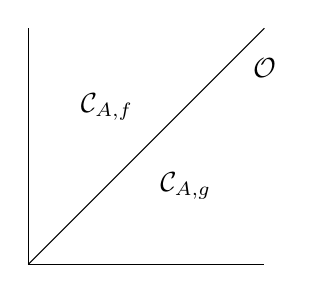
\begin{tikzpicture}
  \draw (0,0)--(0,3);
  \draw (1,2)node{$ \mathcal{C}_{A,f} $};
  \draw (0,0)--(3,0);
  \draw (2,1)node{$ \mathcal{C}_{A,g} $};
  \draw(0,0)--(3,3);
  \draw(3,2.5)node{$ \mathcal{O} $};
\end{tikzpicture}
$\qquad\qquad\qquad\qquad$or$\qquad\qquad\qquad\qquad$
\begin{tikzpicture}
  \draw (0,0)--(0,3);
  \draw (1,2)node{$ \mathcal{C}_{A,f} $};
  \draw(0,0)--(3,3);
  \draw(3,1.5)node{$ \mathcal{O}= \mathcal{C}_{A,g}$};
\end{tikzpicture}
\begin{proof}
 By assumption $f$  is birational and $X$  is $\mathbb{Q}$-factorial. Let $h: W \dashrightarrow S$ be the ample model corresponding to  $K_{W}+D$. Since $D$  is not a point of the boundary of $\mathcal{L}_{A}(V)$,  if $D$ belongs to the boundary of $\mathcal{E}_{A}$ then $K_{W}+D$ is not big and so $h$  is not birational. As $\mathcal{O}$   is a subset of both $\mathcal{C}_{A,f}$ and $\mathcal{C}_{A,g}$ there are morphisms $p: X\to S $ and  $q:Y\to S$ 
of relative Picard number at most one. There are therefore only two cases
\begin{enumerate}
  \item $\rho (X)=\rho(Y)+1$, or 
  \item $\rho(X)=\rho(Y)$
\end{enumerate}
Suppose we are in the first case, then $q$ is the identity and $\pi:X\to Y$  is a contraction morphism such that $
g=p \circ f$. Suppose that $\pi$ is birational, then $ h $ is birational and $\mathcal{O}$ is not contained in the boundary of  $\mathcal{E}_{A}(V)$. If $\pi$ is divisorial then $Y$ is $\mathbb{Q}$-factorial and so $\mathcal{O} \neq \mathcal{C}_{A,g}$. If $\pi $ is a small contraction then $\pi $ is not $\mathbb{Q}$-factorial and so $\mathcal{C}_{A,g}=\mathcal{O}$ is one dimensional. If $\pi $ is a Mori fibre space then $\mathcal{O} $ is contained in the boundary of $\mathcal{E}_{A}(V)$ and $\mathcal{O} = \mathcal{C}_{A,g}$.

Now suppose we are in the second case. Since $\rho(X/S)=\rho(Y/S)=1$, we know that $p,q$ are not divisoriacontractions as $\mathcal{O}$ is one dimensional and $p,q $ are not Mori fibre spaces as $\mathcal{O} $ is cannot be contained in the boundary of $\mathcal{E}_{A}(V)$. Hence  $p,q$ are small and the the rest is clear.
\end{proof}

\begin{lem}
  \cite[Lemma 3.6]{haconSarkisovProgram2011} Let $f:W\dashrightarrow X $ be a birational contraction between $\mathbb{Q}$-factorial varieties. Suppose $(W,D)$ and $(W,D+A)$ are both klt. If $f$ is ample model of $(W,D+A)$ and $A$ is ample, then $f$ is result of running $(K_{W}+D)$-MMP.
\end{lem}
This lemma gunrantee that every variety in the Sarkisov links constructed later is a MMP result of $(W,B_{W})$.

Finally we show there is a Sarkisov link corresponding to certain $D \in \mathcal{E}_{A}(V)$. Let $ D=A+B $ be a point of boundary of $ \mathcal{E}_A(V) $ in the interior of $ \mathcal{L}_A(V) $. Let $ \mathcal{T}_1, \ldots, \mathcal{T}_k $ be the polytopes $ \mathcal{C}_i $ of dimension $ 2 $ containing $ D $. Let $ \mathcal{O}_0 $ and $ \mathcal{O}_k $ be the intersection of $ \mathcal{T}_0 $ and $ \mathcal{T}_k $ with boundary of $ \mathcal{E}_A(V) $, and let $ \mathcal{O}_i=\mathcal{T}_i\cap\mathcal{T}_{i+1} $. Let $ f_i:W\dashrightarrow  X_i $ be the birational contraction associated to $ \mathcal{T}_i $ and $ g_i:W\dashrightarrow  S_i $ be the rational contraction associated to $ \mathcal{O}_i $.

\begin{tikzpicture}
  \draw (0,0)node[below]{$ D $}--(-6,4)node[above]{$ \mathcal{O}_0 $};
  \draw (-2.5,2)node[right]{$ \mathcal{T}_1 $};
  \draw (0,0)--(-1.5,2)node[right]{$ \mathcal{T}_{2} $}--(-3,4)node[above]{$ \mathcal{O}_{2} $};
  \draw (0,0)--(-0.5,2)node[right]{$ \cdots $}--(-1,4);
  \draw (0,0)--(0.5,2)node[right]{$ \mathcal{T}_{k-1} $}--(1,4);
  \draw (0,0)--(3,4)node[above]{$ \mathcal{O}_{k-1} $};
  \draw (2,2)node[right]{$ \mathcal{T}_{k} $};
  \draw (0,0)--(6,4)node[above]{$ \mathcal{O}_{k} $};
\end{tikzpicture}

Set $ f=f_1:W\dashrightarrow X, g=f_k:W\dashrightarrow Y $ and $ \phi:X\to S=S_0,\psi:Y\to T=S_k $ and $ X'=X_2,Y'=X_{k-1} $ and let $ W\dashrightarrow R $ be the ample model of $ D $. Then
\begin{thm}\label{constructlink}
  \cite[Theorem 3.7]{haconSarkisovProgram2011} Suppose $ B_W $ is a divisor such that $ K_Z+B_W $ is klt and $ D-B_W $ is ample. Then $ \phi $ and $ \psi $ are Mori fibre spaces as outputs of $ (K_Z+B_W) $-MMP and connected by a Sarkisov link if $ D $ is contained in more than two polytopes.
\end{thm}
\begin{proof}
  WMA $ k\geqslant 3 $ and we have 
  $$ \xymatrix{
  X'\ar@{.>}[d]_p\ar@{.>}[rr]&&Y'\ar@{.>}[d]^q\\
  X\ar[d]_{\phi}&&Y\ar[d]^\psi\\
  S\ar[rd]^s&&T\ar[ld]_t\\
  &R&} $$
Note that $ \rho(X_i/R)\leqslant 2 $ and $ \rho(X/S)=\rho(Y/T)=1 $. Thus 
\begin{enumerate}
  \item $ s $ is identity and $ p $ is a divisorial contraction (extraction), or
  \item $ s $ is a contraction and $ p $ is a flop.
\end{enumerate}
The same holds for $ q $ and $ t $. And the map $X'\to Y'$ is clear the composition of flops. This gives 4 types of links.
\end{proof}
\subsection{Decomposition of $\Phi$}
We need a special resolution $W$ and a special  affine subspace $V \subset \operatorname{WDiv}(W)$.
\begin{lem}\label{keylemma}
  \cite[Lemma 4.1]{haconSarkisovProgram2011} Let $ \phi:X\to S $ and $ \psi :Y\to T  $ be two MMP related Mori fibre space corresponding to two klt projective varieties $ (X,B_X) $ and $ (Y,B_Y) $. Then we may find a smooth projective variety $ W $, two biratinal morphism $ f:W\to X $ and $ g:W\to Y $, a klt pair $ (W,B_{W}) $, an ample $ \mathbb{Q} $-divisor $ A $ on $ W $ and a two dimensional rational affine subspace $ V $ of $ \mathrm{WDiv}_\mathbb{R}(W) $ such that 
  \begin{enumerate}
    \item If $ D\in \mathcal{L}_A(V) $ then $ D-B_W $ is ample;
    \item $ \mathcal{A}_{A,\phi\circ f} $ and $ \mathcal{A}_{A,\psi\circ g} $ are not contained in the boundary of $ \mathcal{L}_A(V) $;
    \item $ V $ satisfy \ref{mapbetweenAM};
    \item $ \mathcal{C}_{A,f} $ and $ \mathcal{C}_{A,g} $ are two dimensional;
    \item $ \mathcal{C}_{A,\phi\circ f} $ and $ \mathcal{C}_{A,\psi\circ g} $ are one dimensional.
  \end{enumerate}
\end{lem}
\begin{proof}
  By assumption there is a $\mathbb{Q}$-factorial klt pair $(W,B_{W})$ such that $f:W\dashrightarrow X$ and $g:W \dashrightarrow Y$are both outcomes of $(K_{W}+B_{W})$-MMP. Let $p':W'\to W$ be any log resolution such that resolves the indeterminacy of $f$ and $g$, then we may write
  \[
    K_{W'}+B_{W'}=p'^*(K_{W}+B_{W})+E'
  \]
where $E'\geqslant 0$ and $B_{W'}\geqslant 0$ have no common components, and $E'$ is exceptional and $p'_*B_{W'}=B_{W}$. Pick a divisor $-F$ which is ample over $W$ with support equal to the full exceptional locus such that $K_{W'}+B_{W'}+F$ is klt. As $p'$ is $(K_{W'}
B_{W'}+F)$-negative and $(K_{W}+B_{W})$ is klt and $W$ is $\mathbb{Q}$-factorial, the $(K_{W'}+B_{W'}+F)$-MMP over $W$ terminates with the pair $(W,B_{W})$. Replacing $(W,B_{W})$ by $(W',B_{W'} +F)$ we may assume that $(W,B_{W})$ is log smooth and $f,g$ are morphisms.

Pick general ample $\mathbb{Q}$-divisors $A, H_{1},H_{2},\ldots ,H_{k}$ on $W$ such that $H_{1},\ldots , H_{k}$ generate te Neron-Severi group of $W$. Let $H=A+H_{1}+\ldots+ H_{k}$. Pick sufficiently ample divisor $A_{S}$ on $S$ and $A_{T}$ on $T$ such that
\[
-(K_{X}+B_{X})+\phi^*A_{S} \text{ and } -(K_{Y}+B_{Y})\psi^*A_{T}
\]
are both ample. Pick a rational number $0<\delta<1$ such that 
\[
  -(K_{X}+B_{X}+\delta f_*H)+\phi^*A_{S} \text{ and } -(K_{Y}+B_{Y}+\delta g_*H)+\psi^*A_{T}
\]
are both ample and $(K_{W}+B_{W}+\delta H)$ is both  $f$ and  $g$ negative. Replacing $H$ by $\delta H$ we may assume that $\delta=1$. Now pick a $\mathbb{Q}$-divisor $B_{0}\leqslant B_{W}$ such that $A+(B_{0}-B_{W}), -(K_{X}+ f_*B_{0}+f_*H)+\phi^*A_{S}$ and $-(K_{Y}+ g_*B_{0}+f_*H)+\psi^*A_{T}$  are all ample and $(K_{W}+B_{0}+H)$ is both  $f$ and  $g$ negative.

Pick general ample $\mathbb{Q}$-divisors $F_{1}\geqslant 0$ and $G_{1}\geqslant 0$  such that
\[
F_{1}\sim_{\mathbb{Q}} -(K_{X}+f_*B_{0}+ f_*H)+\phi^*A_{S} \text{ and } G_{1}\sim_{\mathbb{Q}} -(K_{Y}+g_*B_{0}+ g_*H)+\psi^*A_{T}
\]
and 
\[
  K_{W}+B_{0}+H+F+G
\]
is klt, where $F=f^*F_{1}$ and $G=g^*G_{1}$. 

Let $V_{0}$ be the affine subspace of $\operatorname{WDiv}_{\mathbb{R}}(W)$ which is the translate by $B_{0}$ of the vector subspace  spaned by $H_{1},\ldots , H_{k},F,G$. Supppose that $D=A+B \in \mathcal{L}_{A}(V_{0})$. Then 
\[
  D-B_W=(A+B_{0}-B_{W})+(B-B_{0})
\]
is ample, as $B-B_{0}$ is nef by definition of $V_{0}$. Note the 
\[
  B_{0}+F+H \in \mathcal{A}_{A,\phi\circ f}(V_{0}), B_{0}+G+H \in \mathcal{A}_{\psi \circ g}(V_{0})
\]
and $f$, respectively $g$, is a weak log canonical model of $K_{W}+B_{0}+F+H$, respectively $K_{W}+B_{0}+G+H$. Thus theorem \ref{mapbetweenAM} implies that $V_{0}$ satisfies (1-4) of \ref{mapbetweenAM}.

Since $H_{1},\ldots ,H_{k}$ generated the Neron-Severi group of $W$ we may find constants $h_{1},\ldots ,h_{k}$ such that $G \equiv \sum^{k}_{i=1} h_{i}H_{i}$. Then there is $0< \delta\ll 1$ such that  $B_{0}+F+\delta G+H- \delta(\sum_{i=1}^{k} h_{i}H_{i}) \in \mathcal{L}_{A}(V_{0})$ and
\[
  B_{0}+F+\delta G+H-\delta (\sum_i^k h_{i}H_{i}) \equiv B_{0}+F+H
.\]
Thus $\mathcal{A}_{A,\phi\circ f}$ is not contained in the boundary of $\mathcal{L}_{A}(V_{0})$. Similarly $\mathcal{A}_{A,\psi\circ g}$ is not contained in the boundary of $\mathcal{L}_{A}(V_{0})$. In particular $\mathcal{A}_{A,\phi\circ f}$ and   $\mathcal{A}_{A,\psi\circ g}$ span affine hyperplanes of $V_{0}$, since $\rho(X)=\rho(Y)=1$.

Let $V_{1}$ be the translate by $B_{0}$ of two dimensional vector space spaned by $F+H-A$ and $F+G-A$. Let $V$ be a small general perturbation of $V_{1}$, which is defined over rationals. This is the affine subspace we need.
\end{proof}
Then we can prove the main theorem
\begin{proof}[Proof of \ref{main}]
Let $(W,B_{W}),A $ and $V$ as in the lemma \ref{keylemma}.  Pick $ D_{0} \in \mathcal{A}_{A,\phi\circ f} $  and $ D_1\in \mathcal{C}_{A,g} $ belonging to the interior of $ \mathcal{L}_A(V) $. As $ V $ is two dimensional, removing $ D_0 $ and $ D_1 $ divides the boundary of $ \mathcal{E}_A(V) $ into two parts. The part which consists entirely of divisors which are not big is contained in the interior of $ \mathcal{L}_A(V) $. Consider tracing this boundary from $ D_0 $ to $ D_1 $. Then there are finitely many $ 2\leqslant i\leqslant N $ points $ D_i $ which are contained in more than two polytopes $ \mathcal{C}_{A,f_i}(V) $. By lemma \ref{constructlink},  each point $ D_i $ gives a Sarkisov link. And the birational map $X \dashrightarrow Y$ is composition of such links.
\end{proof}

\section{Examples}
% TODO: compute an example

\section{Application}

\bibliographystyle{plain}
\bibliography{ref}

\end{document}
